\chapter{Phân tích nhiều chiều dữ liệu thang đo định lượng}

Phân tích dữ liệu nhiều chiều là một lĩnh vực quan trọng của thống kê hiện đại, cho phép chúng ta khám phá và hiểu mối quan hệ phức tạp giữa nhiều biến số đồng thời. Chương này sẽ trình bày các kỹ thuật cơ bản và nâng cao trong phân tích nhiều chiều, từ những khái niệm cơ sở đến các ứng dụng thực tiễn.

\section{Khái niệm cơ bản về dữ liệu nhiều chiều}

\subsection{Vector ngẫu nhiên và phân phối nhiều chiều}
\begin{dn}[Vector ngẫu nhiên]
Vector ngẫu nhiên $p$-chiều là một ánh xạ $\mathbf{X}: \Omega \to \mathbb{R}^p$ được viết dưới dạng
\[
\mathbf{X} = \begin{pmatrix} X_1 \\ X_2 \\ \vdots \\ X_p \end{pmatrix}
\]
trong đó mỗi $X_i$ là một biến ngẫu nhiên.
\end{dn}

\subsection{Vector kỳ vọng và ma trận hiệp phương sai}
\begin{dn}[Vector kỳ vọng]
\[
\boldsymbol{\mu} = \mathbb{E}[\mathbf{X}] = \begin{pmatrix} \mathbb{E}[X_1] \\ \mathbb{E}[X_2] \\ \vdots \\ \mathbb{E}[X_p] \end{pmatrix}
\]
\end{dn}

\begin{dn}[Ma trận hiệp phương sai]
\[
\boldsymbol{\Sigma} = \Cov(\mathbf{X}) = \mathbb{E}[(\mathbf{X} - \boldsymbol{\mu})(\mathbf{X} - \boldsymbol{\mu})^T]
\]
với phần tử thứ $(i,j)$ là $\Sigma_{ij} = \Cov(X_i, X_j)$.
\end{dn}

\begin{tinhchat}[Tính chất của ma trận hiệp phương sai]
\begin{itemize}
    \item $\boldsymbol{\Sigma}$ là ma trận đối xứng: $\boldsymbol{\Sigma} = \boldsymbol{\Sigma}^T$
    \item $\boldsymbol{\Sigma}$ là ma trận nửa xác định dương
    \item Đường chéo chính chứa các phương sai: $\Sigma_{ii} = \Var(X_i)$
\end{itemize}
\end{tinhchat}

\subsection{Phân phối chuẩn nhiều chiều}
\begin{dn}[Phân phối chuẩn nhiều chiều]
Vector ngẫu nhiên $\mathbf{X}$ có phân phối chuẩn nhiều chiều $\mathcal{N}_p(\boldsymbol{\mu}, \boldsymbol{\Sigma})$ nếu có hàm mật độ:
\[
f(\mathbf{x}) = \frac{1}{(2\pi)^{p/2}|\boldsymbol{\Sigma}|^{1/2}} \exp\left(-\frac{1}{2}(\mathbf{x} - \boldsymbol{\mu})^T\boldsymbol{\Sigma}^{-1}(\mathbf{x} - \boldsymbol{\mu})\right)
\]
\end{dn}

\section{Ma trận tương quan và các đặc trưng mô tả}

\subsection{Ma trận tương quan}
\begin{dn}[Ma trận tương quan]
Ma trận tương quan $\mathbf{R}$ có phần tử thứ $(i,j)$ là:
\[
\rho_{ij} = \frac{\Cov(X_i, X_j)}{\sqrt{\Var(X_i)\Var(X_j)}} = \frac{\Sigma_{ij}}{\sqrt{\Sigma_{ii}\Sigma_{jj}}}
\]
\end{dn}

Mối quan hệ giữa ma trận hiệp phương sai và ma trận tương quan:
\[
\boldsymbol{\Sigma} = \mathbf{D}^{1/2} \mathbf{R} \mathbf{D}^{1/2}
\]
trong đó $\mathbf{D} = \text{diag}(\Sigma_{11}, \Sigma_{22}, \ldots, \Sigma_{pp})$.

\subsection{Ước lượng mẫu}
Với mẫu $\mathbf{x}_1, \mathbf{x}_2, \ldots, \mathbf{x}_n$:

\textbf{Vector trung bình mẫu:}
\[
\overline{\mathbf{x}} = \frac{1}{n}\sum_{i=1}^n \mathbf{x}_i
\]

\textbf{Ma trận hiệp phương sai mẫu:}
\[
\mathbf{S} = \frac{1}{n-1}\sum_{i=1}^n (\mathbf{x}_i - \overline{\mathbf{x}})(\mathbf{x}_i - \overline{\mathbf{x}})^T
\]

\textbf{Ma trận tương quan mẫu:}
\[
\mathbf{R} = \mathbf{D}_S^{-1/2} \mathbf{S} \mathbf{D}_S^{-1/2}
\]
với $\mathbf{D}_S = \text{diag}(S_{11}, S_{22}, \ldots, S_{pp})$.

\section{Phân tích thành phần chính (Principal Component Analysis - PCA)}

\subsection{Động lực và ý tưởng cơ bản}
PCA là kỹ thuật giảm chiều dữ liệu bằng cách tìm các hướng có phương sai lớn nhất. Mục tiêu là chuyển đổi dữ liệu gốc $p$-chiều thành không gian mới có chiều thấp hơn mà vẫn giữ được nhiều thông tin nhất.

\subsection{Định nghĩa toán học}
\begin{dn}[Thành phần chính thứ nhất]
Thành phần chính thứ nhất là tổ hợp tuyến tính $Y_1 = \mathbf{a}_1^T\mathbf{X}$ sao cho:
\begin{itemize}
    \item $\Var(Y_1) = \mathbf{a}_1^T\boldsymbol{\Sigma}\mathbf{a}_1$ đạt giá trị lớn nhất
    \item Ràng buộc: $\|\mathbf{a}_1\| = 1$
\end{itemize}
\end{dn}

\begin{dl}[Nghiệm của bài toán PCA]
Các thành phần chính được xác định thông qua phân tích trị riêng của ma trận hiệp phương sai:
\[
\boldsymbol{\Sigma}\mathbf{a}_i = \lambda_i\mathbf{a}_i, \quad i = 1, 2, \ldots, p
\]
với $\lambda_1 \geq \lambda_2 \geq \cdots \geq \lambda_p \geq 0$ và $\|\mathbf{a}_i\| = 1$.
\end{dl}

\subsection{Tính chất quan trọng}
\begin{tinhchat}[Tính chất của PCA]
\begin{itemize}
    \item Phương sai của thành phần chính thứ $i$: $\Var(Y_i) = \lambda_i$
    \item Tổng phương sai được bảo toàn: $\sum_{i=1}^p \lambda_i = \sum_{i=1}^p \Var(X_i)$
    \item Các thành phần chính không tương quan: $\Cov(Y_i, Y_j) = 0$ với $i \neq j$
    \item Tỷ lệ phương sai được giải thích bởi $k$ thành phần đầu: $\frac{\sum_{i=1}^k \lambda_i}{\sum_{i=1}^p \lambda_i}$
\end{itemize}
\end{tinhchat}

\subsection{Thuật toán thực hiện PCA}
\begin{enumerate}
    \item \textbf{Chuẩn hóa dữ liệu}: Chuyển về dạng $Z$-score nếu cần
    \item \textbf{Tính ma trận hiệp phương sai} (hoặc tương quan)
    \item \textbf{Phân tích trị riêng}: Tìm $\lambda_i$ và $\mathbf{a}_i$
    \item \textbf{Sắp xếp}: Theo thứ tự giảm dần của $\lambda_i$
    \item \textbf{Chọn số thành phần}: Dựa trên tiêu chí phù hợp
    \item \textbf{Chuyển đổi dữ liệu}: $\mathbf{Y} = \mathbf{A}^T\mathbf{X}$
\end{enumerate}

\subsection{Tiêu chí lựa chọn số thành phần}
\subsubsection*{Tiêu chí Kaiser}
Giữ lại các thành phần có $\lambda_i > 1$ (khi sử dụng ma trận tương quan).

\subsubsection*{Tiêu chí phần trăm phương sai}
Chọn $k$ sao cho $\frac{\sum_{i=1}^k \lambda_i}{\sum_{i=1}^p \lambda_i} \geq 0.80$ (hoặc 0.85, 0.90).

\subsubsection*{Scree plot}
Vẽ đồ thị $\lambda_i$ theo $i$ và tìm "điểm khuỷu" (elbow point).

\subsection{Ví dụ minh họa với MATLAB}
\begin{matlab}
\begin{lstlisting}
function [scores, coeff, latent, explained] = pca_analysis(X)
% Phân tích thành phần chính
% INPUT: X - ma trận dữ liệu (n x p)
% OUTPUT: scores - điểm số PC, coeff - hệ số, latent - trị riêng, 
%         explained - phần trăm phương sai giải thích

% Chuẩn hóa dữ liệu
X_std = zscore(X);

% PCA
[coeff, scores, latent] = pca(X_std);

% Tính phần trăm phương sai giải thích
explained = 100 * latent / sum(latent);

% Vẽ scree plot
figure;
subplot(1,2,1);
plot(1:length(latent), latent, 'bo-', 'LineWidth', 2);
xlabel('Thành phần chính');
ylabel('Trị riêng');
title('Scree Plot');
grid on;

% Vẽ phần trăm tích lũy
subplot(1,2,2);
plot(1:length(explained), cumsum(explained), 'ro-', 'LineWidth', 2);
xlabel('Thành phần chính');
ylabel('Phần trăm tích lũy (%)');
title('Phương sai tích lũy');
grid on;
ylim([0 100]);

% In kết quả
fprintf('Phần trăm phương sai giải thích:\n');
for i = 1:min(5, length(explained))
    fprintf('PC%d: %.2f%% (tích lũy: %.2f%%)\n', ...
        i, explained(i), sum(explained(1:i)));
end
end
\end{lstlisting}
\end{matlab}

\section{Phân tích nhân tố (Factor Analysis)}

\subsection{Mô hình nhân tố}
\begin{dn}[Mô hình nhân tố]
Mô hình nhân tố biểu diễn vector quan sát $\mathbf{X}$ dưới dạng:
\[
\mathbf{X} = \boldsymbol{\mu} + \mathbf{L}\mathbf{F} + \boldsymbol{\epsilon}
\]
trong đó:
\begin{itemize}
    \item $\mathbf{F}$ là vector nhân tố chung $(m \times 1)$ với $m < p$
    \item $\mathbf{L}$ là ma trận tải nhân tố $(p \times m)$
    \item $\boldsymbol{\epsilon}$ là vector sai số cụ thể $(p \times 1)$
\end{itemize}
\end{dn}

\subsection{Giả định của mô hình}
\begin{itemize}
    \item $\mathbb{E}[\mathbf{F}] = \mathbf{0}$ và $\Cov(\mathbf{F}) = \mathbf{I}_m$
    \item $\mathbb{E}[\boldsymbol{\epsilon}] = \mathbf{0}$ và $\Cov(\boldsymbol{\epsilon}) = \boldsymbol{\Psi}$ (ma trận chéo)
    \item $\Cov(\mathbf{F}, \boldsymbol{\epsilon}) = \mathbf{0}$
\end{itemize}

\subsection{Phân tích ma trận hiệp phương sai}
Từ mô hình nhân tố, ta có:
\[
\boldsymbol{\Sigma} = \mathbf{L}\mathbf{L}^T + \boldsymbol{\Psi}
\]

\textbf{Phương sai chung (communality):} $h_i^2 = \sum_{j=1}^m L_{ij}^2$

\textbf{Phương sai cụ thể (specific variance):} $\psi_i = \Sigma_{ii} - h_i^2$

\subsection{Phương pháp ước lượng}
\subsubsection*{Phương pháp thành phần chính}
Sử dụng $m$ thành phần chính đầu tiên để ước lượng ma trận tải:
\[
\hat{\mathbf{L}} = \mathbf{A}_m\boldsymbol{\Lambda}_m^{1/2}
\]
với $\mathbf{A}_m$ chứa $m$ vector riêng đầu và $\boldsymbol{\Lambda}_m = \text{diag}(\lambda_1, \ldots, \lambda_m)$.

\subsubsection*{Phương pháp maximum likelihood}
Tối đa hóa hàm likelihood dưới giả định phân phối chuẩn.

\subsection{Xoay nhân tố (Factor Rotation)}
Mục đích: Tìm ma trận tải dễ giải thích hơn thông qua phép xoay.

\subsubsection*{Xoay Varimax}
Tối đa hóa tổng phương sai của bình phương các tải trong mỗi nhân tố:
\[
V = \sum_{j=1}^m \left[\sum_{i=1}^p L_{ij}^4 - \frac{1}{p}\left(\sum_{i=1}^p L_{ij}^2\right)^2\right]
\]

\subsubsection*{Xoay Promax}
Cho phép các nhân tố tương quan với nhau (oblique rotation).

\section{Phân tích tương quan chính tắc (Canonical Correlation Analysis)}

\subsection{Bài toán tương quan chính tắc}
Cho hai tập biến $\mathbf{X}^{(1)}$ $(p_1 \times 1)$ và $\mathbf{X}^{(2)}$ $(p_2 \times 1)$, tìm các tổ hợp tuyến tính:
\[
U = \mathbf{a}^T\mathbf{X}^{(1)}, \quad V = \mathbf{b}^T\mathbf{X}^{(2)}
\]
sao cho $\Cor(U, V)$ đạt giá trị lớn nhất.

\subsection{Nghiệm toán học}
\begin{dl}[Tương quan chính tắc]
Các tương quan chính tắc $\rho_1 \geq \rho_2 \geq \cdots \geq \rho_r \geq 0$ (với $r = \min(p_1, p_2)$) là căn bậc hai của các trị riêng của ma trận:
\[
\boldsymbol{\Sigma}_{11}^{-1}\boldsymbol{\Sigma}_{12}\boldsymbol{\Sigma}_{22}^{-1}\boldsymbol{\Sigma}_{21}
\]
\end{dl}

\subsection{Ứng dụng và giải thích}
\begin{itemize}
    \item Khám phá mối liên hệ giữa hai nhóm biến
    \item Giảm chiều dữ liệu có cấu trúc phân nhóm
    \item Dự đoán một nhóm biến từ nhóm biến khác
\end{itemize}

\section{Phân tích cụm (Cluster Analysis)}

\subsection{K-means Clustering}
\begin{dl}[Thuật toán K-means]
\begin{enumerate}
    \item Chọn số cụm $k$ và khởi tạo ngẫu nhiên $k$ tâm cụm
    \item Gán mỗi điểm dữ liệu vào cụm có tâm gần nhất
    \item Cập nhật tâm cụm = trung bình của các điểm trong cụm
    \item Lặp lại bước 2-3 đến khi hội tụ
\end{enumerate}
\end{dl}

\textbf{Hàm mục tiêu:} $J = \sum_{i=1}^n \sum_{j=1}^k w_{ij}\|\mathbf{x}_i - \boldsymbol{\mu}_j\|^2$

\subsection{Clustering phân cấp}
\subsubsection*{Agglomerative (Bottom-up)}
\begin{enumerate}
    \item Bắt đầu: mỗi điểm là một cụm
    \item Tại mỗi bước: gộp hai cụm gần nhất
    \item Kết thúc: tất cả điểm trong một cụm
\end{enumerate}

\textbf{Các tiêu chí khoảng cách giữa cụm:}
\begin{itemize}
    \item Single linkage: $d_{min}(C_i, C_j) = \min_{x \in C_i, y \in C_j} d(x,y)$
    \item Complete linkage: $d_{max}(C_i, C_j) = \max_{x \in C_i, y \in C_j} d(x,y)$
    \item Average linkage: $d_{avg}(C_i, C_j) = \frac{1}{|C_i||C_j|}\sum_{x \in C_i}\sum_{y \in C_j} d(x,y)$
    \item Ward linkage: Tối thiểu hóa tổng bình phương sai lệch trong cụm
\end{itemize}

\section{Phân tích phân biệt (Discriminant Analysis)}

\subsection{Phân tích phân biệt tuyến tính (LDA)}
\begin{dn}[Mô hình LDA]
Giả sử có $g$ nhóm với vector trung bình $\boldsymbol{\mu}_i$ và ma trận hiệp phương sai chung $\boldsymbol{\Sigma}$. Hàm phân biệt tuyến tính:
\[
L_i(\mathbf{x}) = \mathbf{x}^T\boldsymbol{\Sigma}^{-1}\boldsymbol{\mu}_i - \frac{1}{2}\boldsymbol{\mu}_i^T\boldsymbol{\Sigma}^{-1}\boldsymbol{\mu}_i + \ln(\pi_i)
\]
với $\pi_i$ là xác suất tiên nghiệm của nhóm $i$.
\end{dn}

\textbf{Quy tắc phân loại:} Gán $\mathbf{x}$ vào nhóm $i$ nếu $L_i(\mathbf{x}) = \max_j L_j(\mathbf{x})$.

\subsection{Phân tích phân biệt bậc hai (QDA)}
Khi các nhóm có ma trận hiệp phương sai khác nhau $\boldsymbol{\Sigma}_i$:
\[
Q_i(\mathbf{x}) = -\frac{1}{2}(\mathbf{x} - \boldsymbol{\mu}_i)^T\boldsymbol{\Sigma}_i^{-1}(\mathbf{x} - \boldsymbol{\mu}_i) - \frac{1}{2}\ln|\boldsymbol{\Sigma}_i| + \ln(\pi_i)
\]

% Hình minh họa được thay thế bằng logo trường
\begin{figure}[h]
    \centering
    % Hình thứ nhất
    \begin{minipage}{0.45\textwidth}
        \centering
        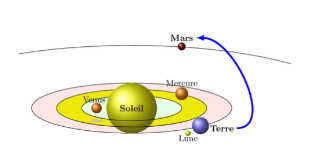
\includegraphics[width=\textwidth]{../../assets/images/figure-2.png}
        \caption{Biểu đồ phân tán dữ liệu đa biến}
        \label{fig:scatter_multivariate}
    \end{minipage}
    \hfill
    % Hình thứ hai
    \begin{minipage}{0.45\textwidth}
        \centering
        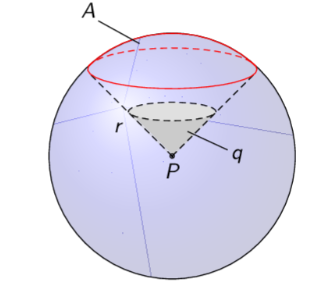
\includegraphics[width=0.8\textwidth]{../../assets/images/figure-3.png}
        \caption{Ma trận tương quan giữa các biến}
        \label{fig:correlation_matrix}
    \end{minipage}
\end{figure}

\begin{figure}[h]
    \centering
    % Hình thứ nhất
    \begin{minipage}{0.45\textwidth}
        \centering
        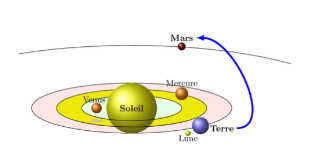
\includegraphics[width=\textwidth]{../../assets/images/figure-2.png}
    \end{minipage}
    \hfill
    % Hình thứ hai
    \begin{minipage}{0.45\textwidth}
        \centering
        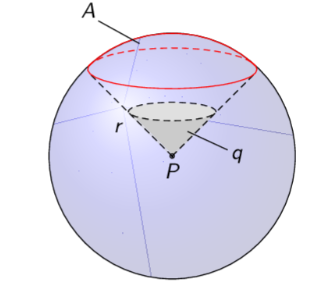
\includegraphics[width=0.8\textwidth]{../../assets/images/figure-3.png}
    \end{minipage}
    \caption{So sánh phương pháp phân tích dữ liệu: (a) Phân tích thành phần chính, (b) Phân tích nhân tố}
    \label{fig:comparison_analysis_methods}
\end{figure}

\section{Ứng dụng tổng hợp và ví dụ thực tiễn}

\subsection{Phân tích dữ liệu kinh tế - xã hội}
Xét bộ dữ liệu về các chỉ số phát triển của các tỉnh thành, bao gồm:
\begin{itemize}
    \item GDP bình quân đầu người
    \item Tỷ lệ biết chữ
    \item Tuổi thọ trung bình
    \item Tỷ lệ thất nghiệp
    \item Chỉ số môi trường
    \item Mật độ dân số
\end{itemize}

\subsubsection*{Quy trình phân tích}
\begin{enumerate}
    \item \textbf{Khám phá dữ liệu}: Ma trận tương quan, biểu đồ phân tán
    \item \textbf{PCA}: Giảm chiều và tìm các nhân tố chính
    \item \textbf{Phân tích cụm}: Nhóm các tỉnh thành có đặc điểm tương tự
    \item \textbf{Phân tích phân biệt}: Xây dựng mô hình phân loại vùng phát triển
\end{enumerate}

\begin{matlab}
\begin{lstlisting}
function analyze_socioeconomic_data(data, province_names, variable_names)
% Phân tích tổng hợp dữ liệu kinh tế - xã hội
% data: ma trận n x p (n tỉnh, p biến)
% province_names: tên các tỉnh
% variable_names: tên các biến

% 1. Khám phá dữ liệu
fprintf('=== THỐNG KÊ MÔ TẢ ===\n');
disp(array2table([mean(data); std(data); min(data); max(data)], ...
    'VariableNames', variable_names, ...
    'RowNames', {'Mean', 'Std', 'Min', 'Max'}));

% Ma trận tương quan
R = corrcoef(data);
figure('Name', 'Ma trận tương quan');
heatmap(variable_names, variable_names, R, ...
    'Colormap', parula, 'ColorbarVisible', 'on');
title('Ma trận tương quan giữa các biến');

% 2. Phân tích thành phần chính
fprintf('\n=== PHÂN TÍCH THÀNH PHẦN CHÍNH ===\n');
[coeff, scores, latent, ~, explained] = pca(zscore(data));

% Scree plot
figure('Name', 'PCA Results');
subplot(2,2,1);
plot(1:length(latent), latent, 'bo-', 'LineWidth', 2);
xlabel('Thành phần chính');
ylabel('Trị riêng');
title('Scree Plot');
grid on;

% Phần trăm phương sai giải thích
subplot(2,2,2);
bar(explained(1:min(5, length(explained))));
xlabel('Thành phần chính');
ylabel('Phần trăm phương sai (%)');
title('Phương sai giải thích');

% Biplot
subplot(2,2,[3,4]);
biplot(coeff(:,1:2), 'Scores', scores(:,1:2), ...
    'VarLabels', variable_names, 'ObsLabels', province_names);
xlabel(['PC1 (' num2str(explained(1), '%.1f') '%)']);
ylabel(['PC2 (' num2str(explained(2), '%.1f') '%)']);
title('Biplot PC1 vs PC2');

% In kết quả PCA
fprintf('Phần trăm phương sai giải thích:\n');
for i = 1:min(4, length(explained))
    fprintf('  PC%d: %.2f%% (tích lũy: %.2f%%)\n', ...
        i, explained(i), sum(explained(1:i)));
end

% 3. Phân tích cụm K-means
fprintf('\n=== PHÂN TÍCH CỤM ===\n');
k_range = 2:6;
silhouette_scores = zeros(size(k_range));

for i = 1:length(k_range)
    k = k_range(i);
    [idx, ~] = kmeans(zscore(data), k, 'Replicates', 10);
    silhouette_scores(i) = mean(silhouette(zscore(data), idx));
end

% Tìm số cụm tối ưu
[~, optimal_k_idx] = max(silhouette_scores);
optimal_k = k_range(optimal_k_idx);

fprintf('Số cụm tối ưu (theo Silhouette): %d\n', optimal_k);

% Phân cụm với k tối ưu
[cluster_idx, centroids] = kmeans(zscore(data), optimal_k, 'Replicates', 20);

% Hiển thị kết quả phân cụm
figure('Name', 'Clustering Results');
subplot(1,2,1);
plot(k_range, silhouette_scores, 'bo-', 'LineWidth', 2);
xlabel('Số cụm');
ylabel('Silhouette Score');
title('Lựa chọn số cụm');
grid on;

subplot(1,2,2);
gscatter(scores(:,1), scores(:,2), cluster_idx);
xlabel(['PC1 (' num2str(explained(1), '%.1f') '%)']);
ylabel(['PC2 (' num2str(explained(2), '%.1f') '%)']);
title(['Kết quả phân cụm (k=' num2str(optimal_k) ')']);
legend('Location', 'best');

% In danh sách từng cụm
for c = 1:optimal_k
    fprintf('\nCụm %d (%d tỉnh):\n', c, sum(cluster_idx == c));
    cluster_provinces = province_names(cluster_idx == c);
    for j = 1:length(cluster_provinces)
        fprintf('  %s\n', cluster_provinces{j});
    end
end

% 4. Đặc trưng từng cụm
fprintf('\n=== ĐặC TRƯNG CÁC CỤM ===\n');
for c = 1:optimal_k
    fprintf('\nCụm %d:\n', c);
    cluster_data = data(cluster_idx == c, :);
    cluster_means = mean(cluster_data);
    
    for v = 1:length(variable_names)
        fprintf('  %s: %.2f ± %.2f\n', variable_names{v}, ...
            cluster_means(v), std(cluster_data(:,v)));
    end
end

end
\end{lstlisting}
\end{matlab}

\subsection{Đánh giá hiệu quả mô hình}
\subsubsection*{Cross-validation cho PCA}
Đánh giá tính ổn định của các thành phần chính thông qua validation chéo.

\subsubsection*{Metrics cho clustering}
\begin{itemize}
    \item \textbf{Silhouette coefficient}: $s_i = \frac{b_i - a_i}{\max(a_i, b_i)}$
    \item \textbf{Calinski-Harabasz index}: $\frac{SS_B/(k-1)}{SS_W/(n-k)}$
    \item \textbf{Davies-Bouldin index}: $\frac{1}{k}\sum_{i=1}^k \max_{j \neq i} \frac{\sigma_i + \sigma_j}{d_{ij}}$
\end{itemize}

\noindent % Để loại bỏ thụt lề đầu dòng
\begin{minipage}{0.4\textwidth} % Phần hình ảnh (40% chiều rộng trang)
    \centering
    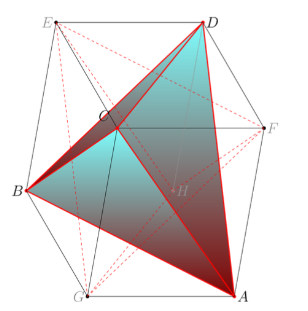
\includegraphics[width=\textwidth]{../../assets/images/figure-1.png} % Đường dẫn tới ảnh
    \captionof{figure}{Quy trình phân tích dữ liệu nhiều chiều} % Chú thích cho hình
    \label{fig:multivariate_workflow}
\end{minipage}%
\hfill % Thêm khoảng cách giữa hình và chữ
\begin{minipage}{0.55\textwidth} % Phần văn bản (55% chiều rộng trang)
    Quy trình phân tích dữ liệu nhiều chiều tổng hợp bao gồm nhiều bước từ khám phá dữ liệu ban đầu đến xây dựng mô hình cuối cùng. Mỗi kỹ thuật có ưu điểm riêng và cần được lựa chọn phù hợp với mục tiêu nghiên cứu cụ thể. Việc kết hợp nhiều phương pháp thường cho kết quả toàn diện và đáng tin cậy hơn.
\end{minipage}

\section{Phân tích nhân tố khám phá (EFA)}

\subsection{Mô hình phân tích nhân tố}

\begin{matlab}
\begin{lstlisting}
function [loadings, eigenvals, explained_var, rotated_loadings] = ...
    exploratory_factor_analysis(data, n_factors, rotation_method)
% EXPLORATORY_FACTOR_ANALYSIS
% Thực hiện phân tích nhân tố khám phá với xoay nhân tố

% Chuẩn hóa dữ liệu
data_std = zscore(data);

% Tính ma trận tương quan
R = corr(data_std);

% Phân tích thành phần chính
[coeff, ~, eigenvals] = pca(data_std);

% Trích n_factors nhân tố đầu tiên
loadings = coeff(:, 1:n_factors) * diag(sqrt(eigenvals(1:n_factors)));

% Tính phần trăm phương sai giải thích
total_var = sum(eigenvals);
explained_var = 100 * eigenvals(1:n_factors) / total_var;

% Xoay nhân tố
switch lower(rotation_method)
    case 'varimax'
        [rotated_loadings, T] = rotatefactors(loadings, 'Method', 'varimax');
    case 'quartimax'
        [rotated_loadings, T] = rotatefactors(loadings, 'Method', 'quartimax');
    otherwise
        rotated_loadings = loadings;
        T = eye(n_factors);
end

% Hiển thị kết quả
fprintf('=== PHÂN TÍCH NHÂN TỐ KHÁM PHÁ ===\n');
fprintf('Số nhân tố: %d\n', n_factors);
fprintf('Phương pháp xoay: %s\n', rotation_method);

communalities = sum(rotated_loadings.^2, 2);
fprintf('\nCommunalities trung bình: %.3f\n', mean(communalities));
end
\end{lstlisting}
\end{matlab}

\begin{figure}[h!]
    \centering
    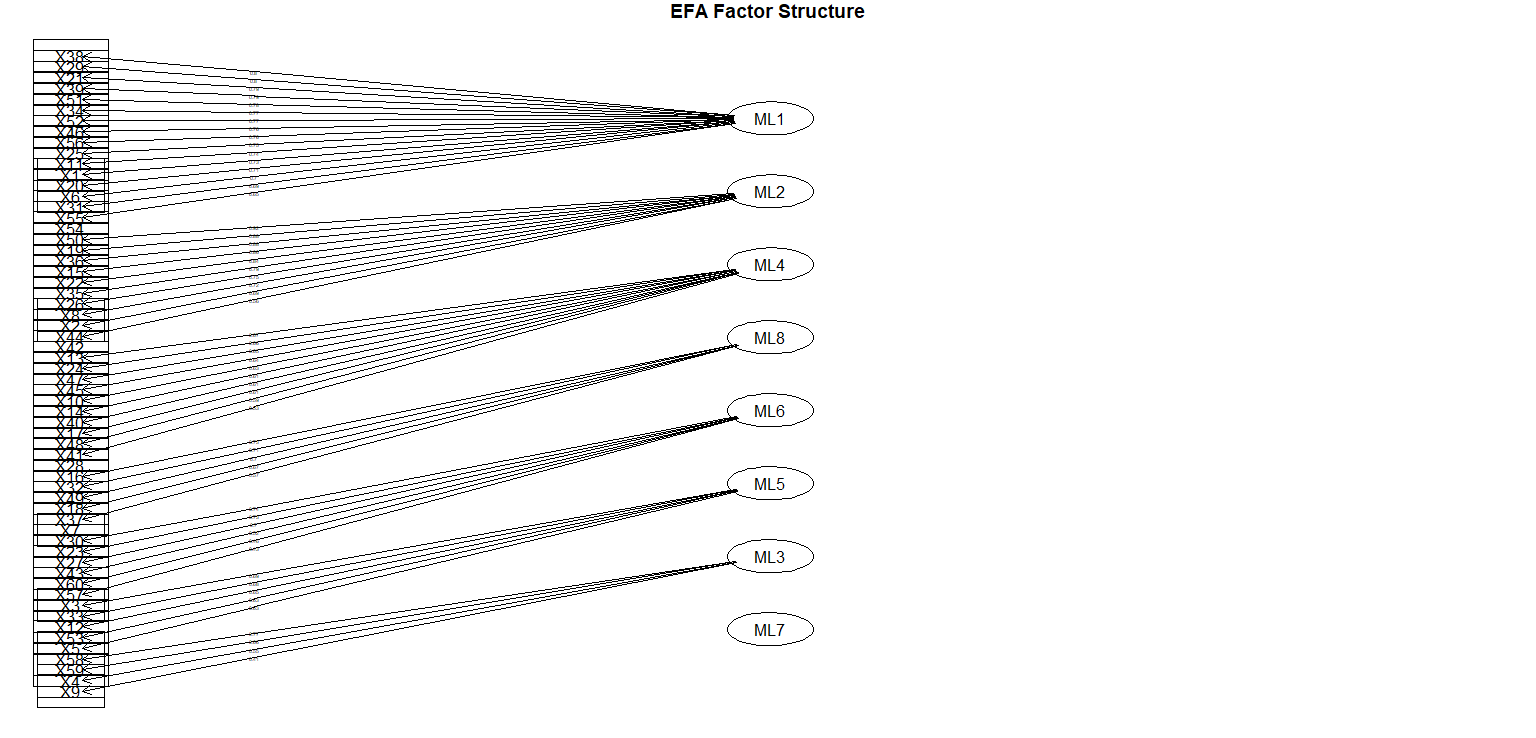
\includegraphics[width=0.8\linewidth]{../../assets/images/EFA_ML.png}
    \caption{Kết quả phân tích nhân tố khám phá với phương pháp Maximum Likelihood}
\end{figure}

\subsection{Kiểm định độ tin cậy Cronbach's Alpha}

\begin{matlab}
\begin{lstlisting}
function alpha = cronbach_alpha(X)
% CRONBACH_ALPHA - Tính hệ số tin cậy Cronbach's Alpha
%
% INPUT: X - ma trận dữ liệu (n x k), k là số biến
% OUTPUT: alpha - hệ số Cronbach's Alpha

[n, k] = size(X);

% Tính phương sai của từng biến
var_items = var(X, 1);

% Tính phương sai của tổng điểm
total_score = sum(X, 2);
var_total = var(total_score, 1);

% Tính Cronbach's Alpha
alpha = (k / (k - 1)) * (1 - sum(var_items) / var_total);

fprintf('Cronbach Alpha = %.4f\n', alpha);
if alpha >= 0.9
    fprintf('Độ tin cậy: Tuyệt vời\n');
elseif alpha >= 0.8
    fprintf('Độ tin cậy: Tốt\n');
elseif alpha >= 0.7
    fprintf('Độ tin cậy: Chấp nhận được\n');
else
    fprintf('Độ tin cậy: Kém\n');
end
end
\end{lstlisting}
\end{matlab}

\begin{figure}[h!]
    \centering
    \begin{minipage}{0.45\textwidth}
        \centering
        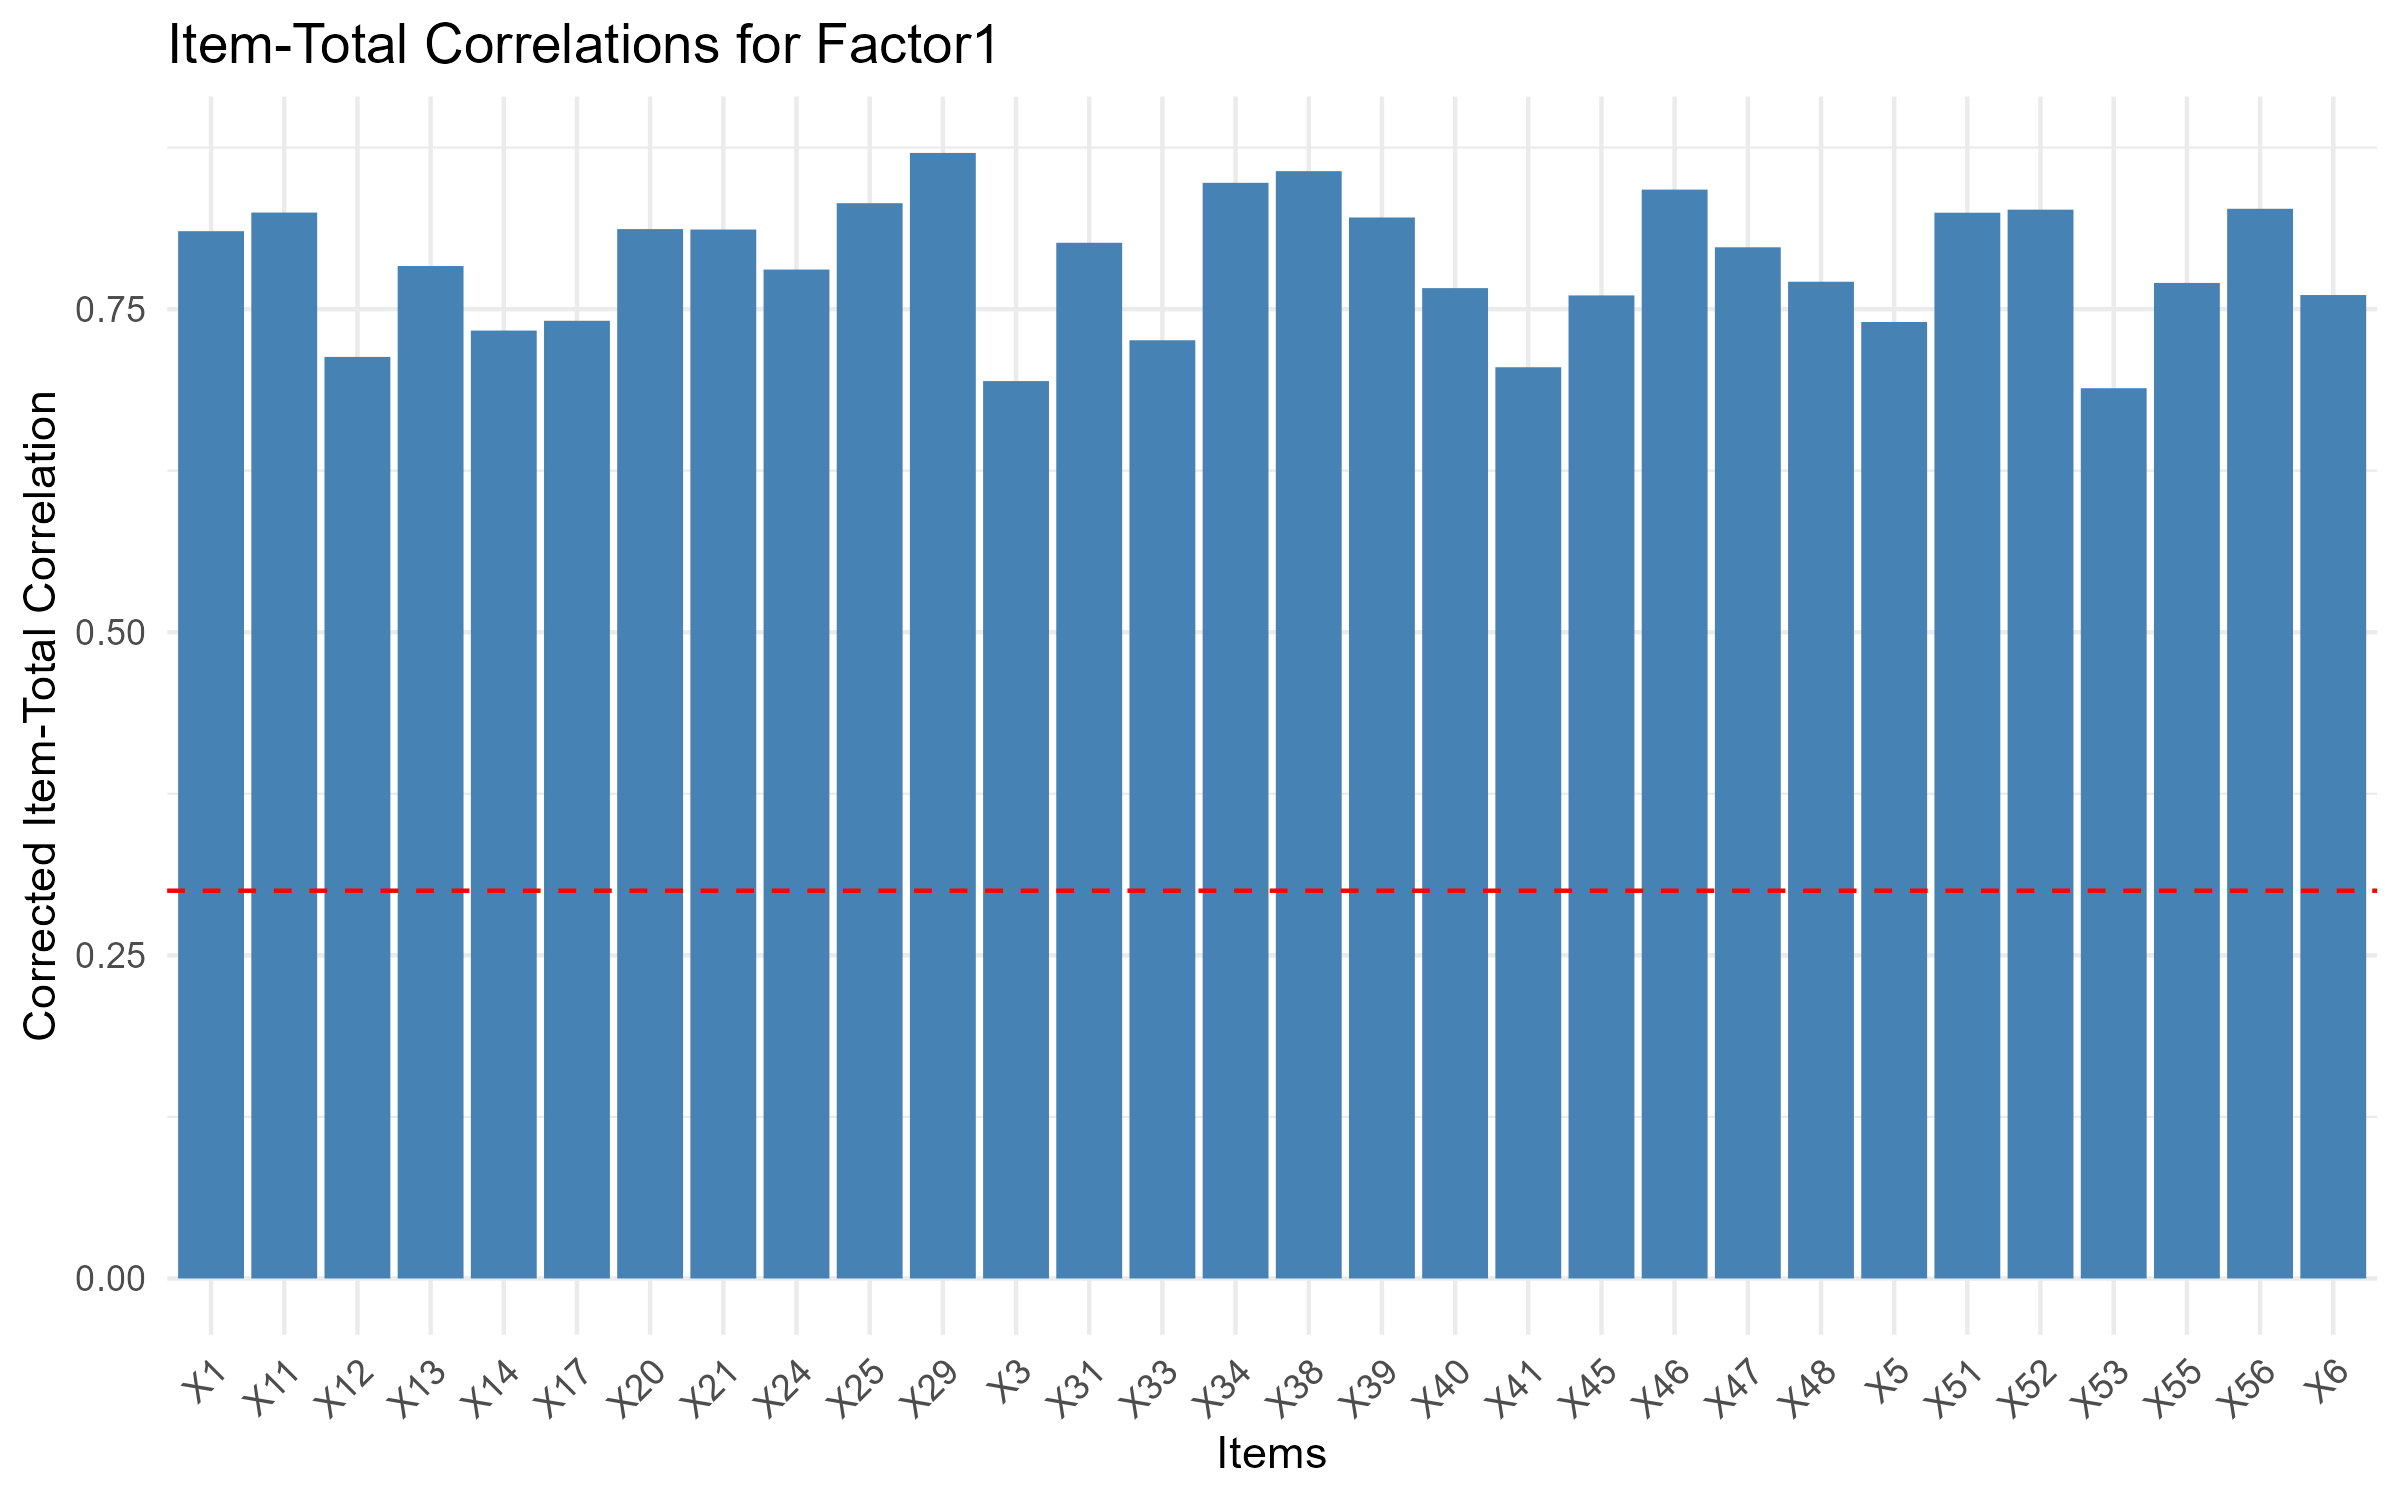
\includegraphics[width=\textwidth]{../../assets/images/reliability_Factor1.png}
        \caption{Độ tin cậy nhân tố 1}
    \end{minipage}
    \hfill
    \begin{minipage}{0.45\textwidth}
        \centering
        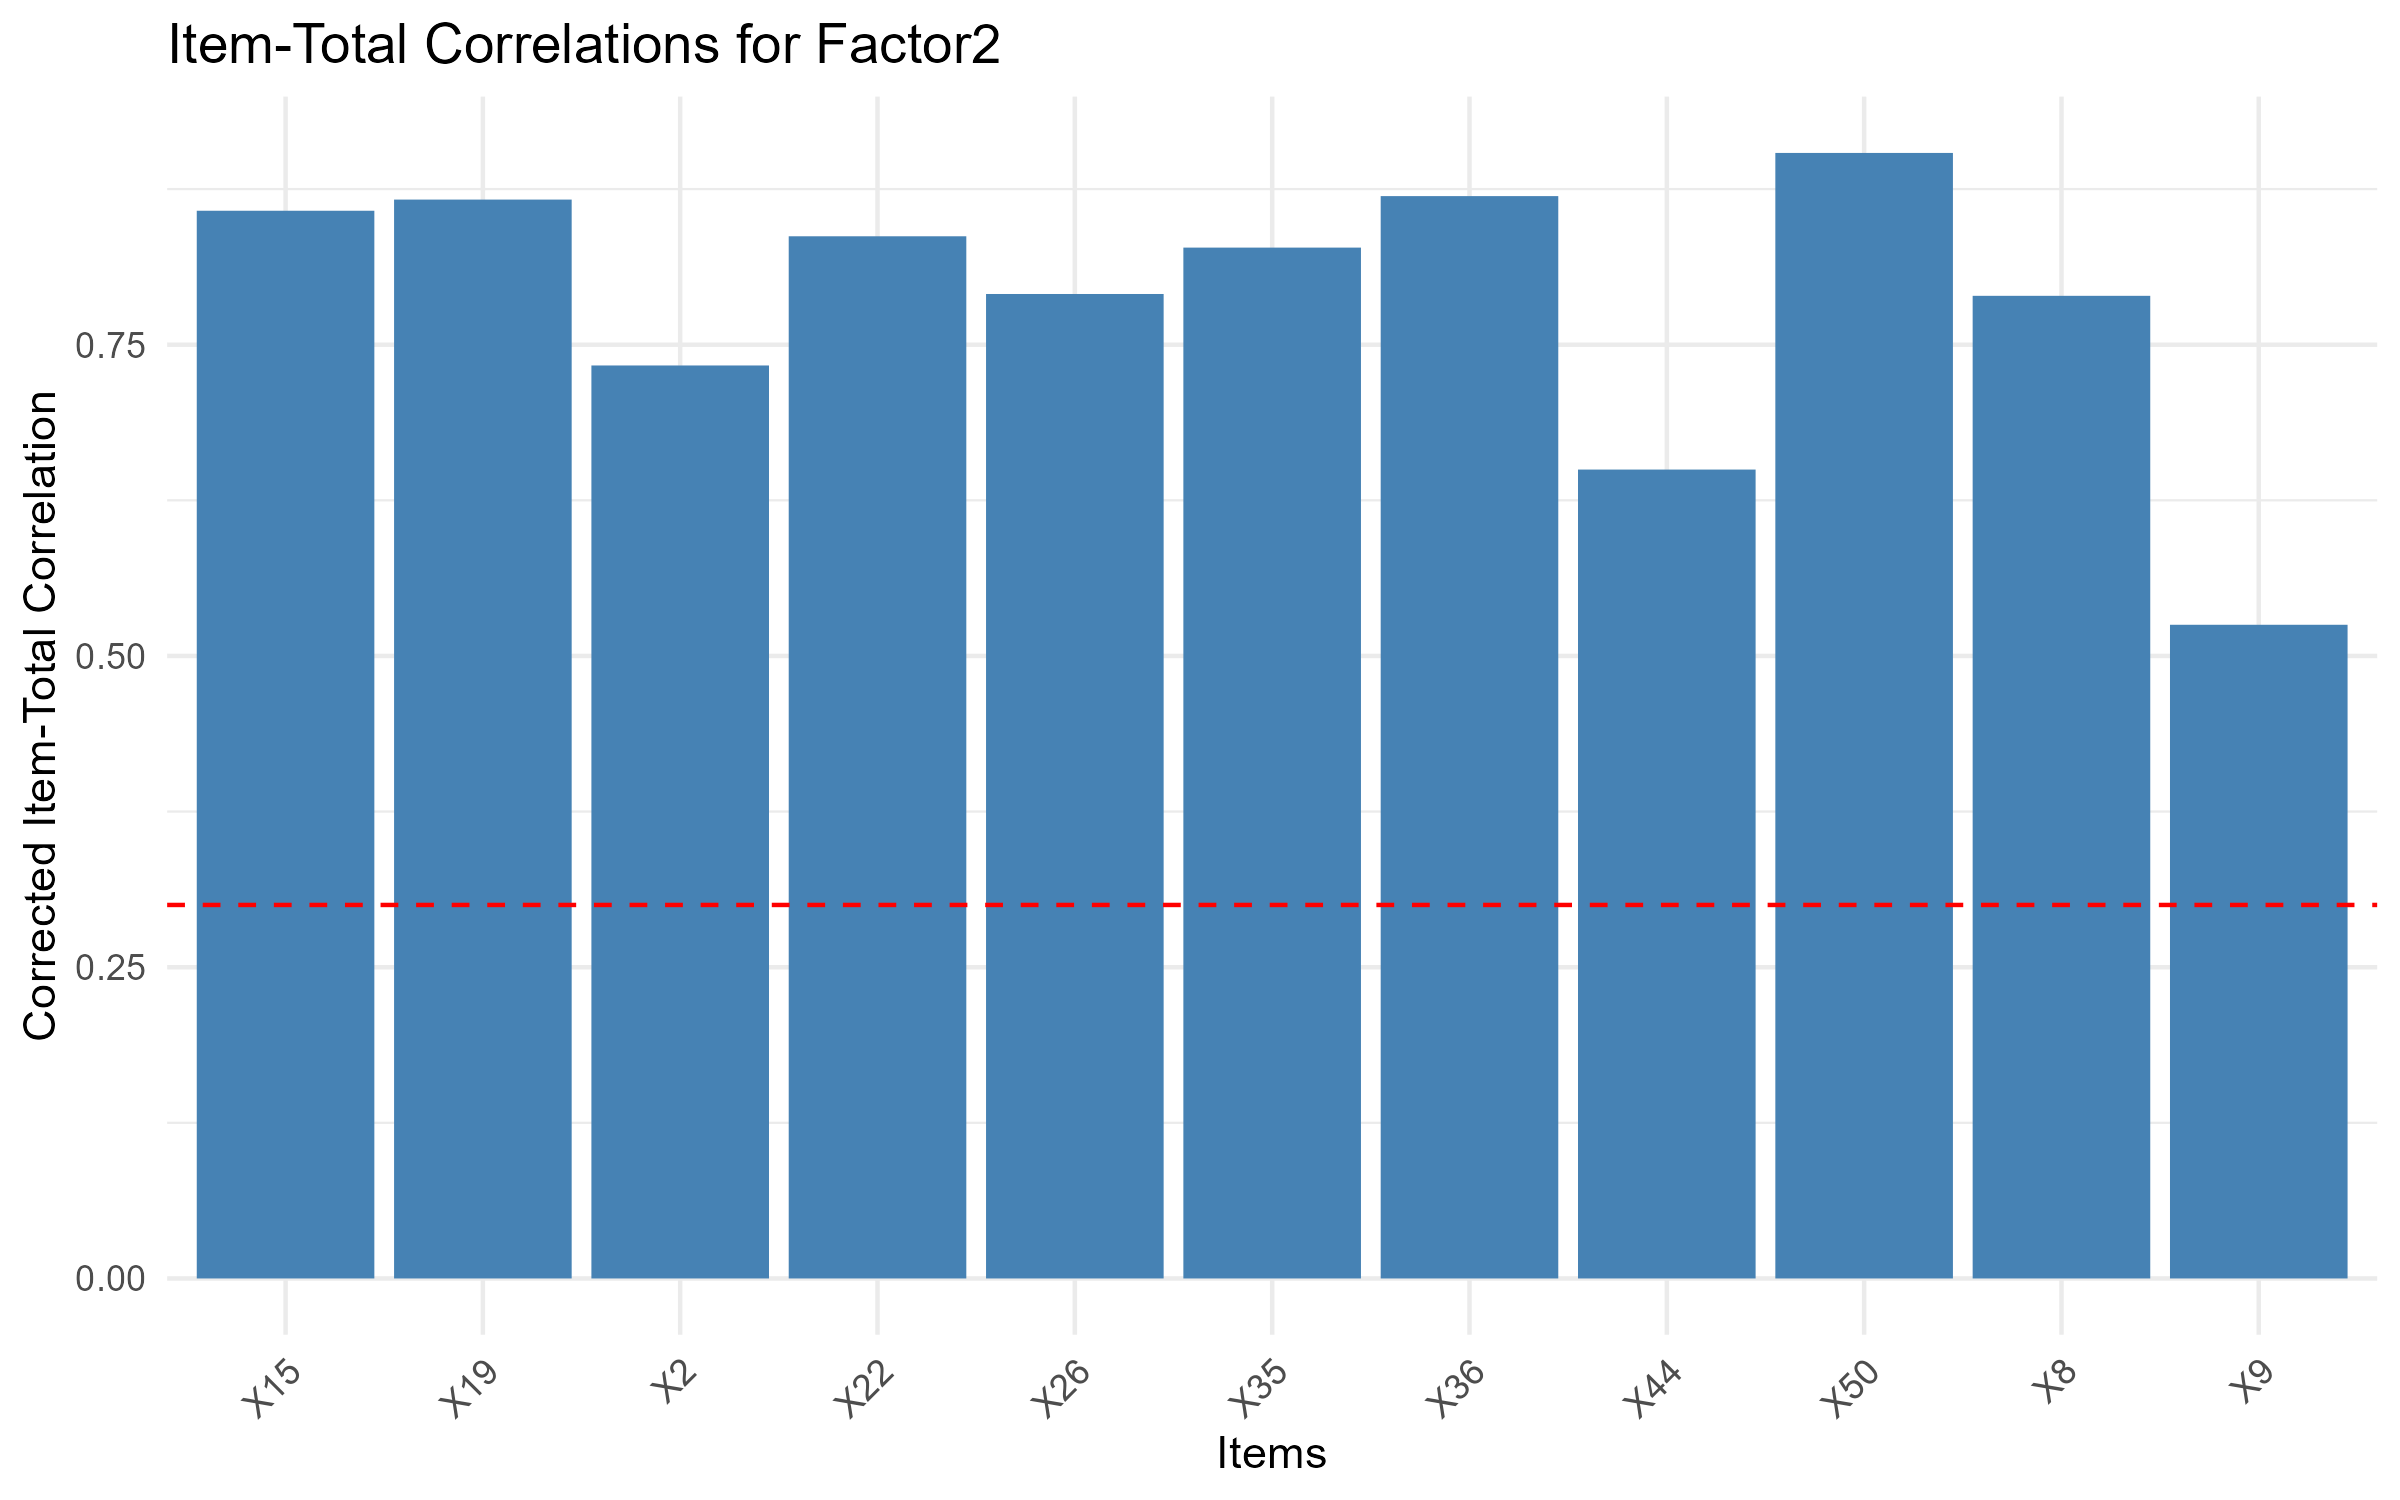
\includegraphics[width=\textwidth]{../../assets/images/reliability_Factor2.png}
        \caption{Độ tin cậy nhân tố 2}
    \end{minipage}
\end{figure}

\begin{figure}[h!]
    \centering
    \begin{minipage}{0.3\textwidth}
        \centering
        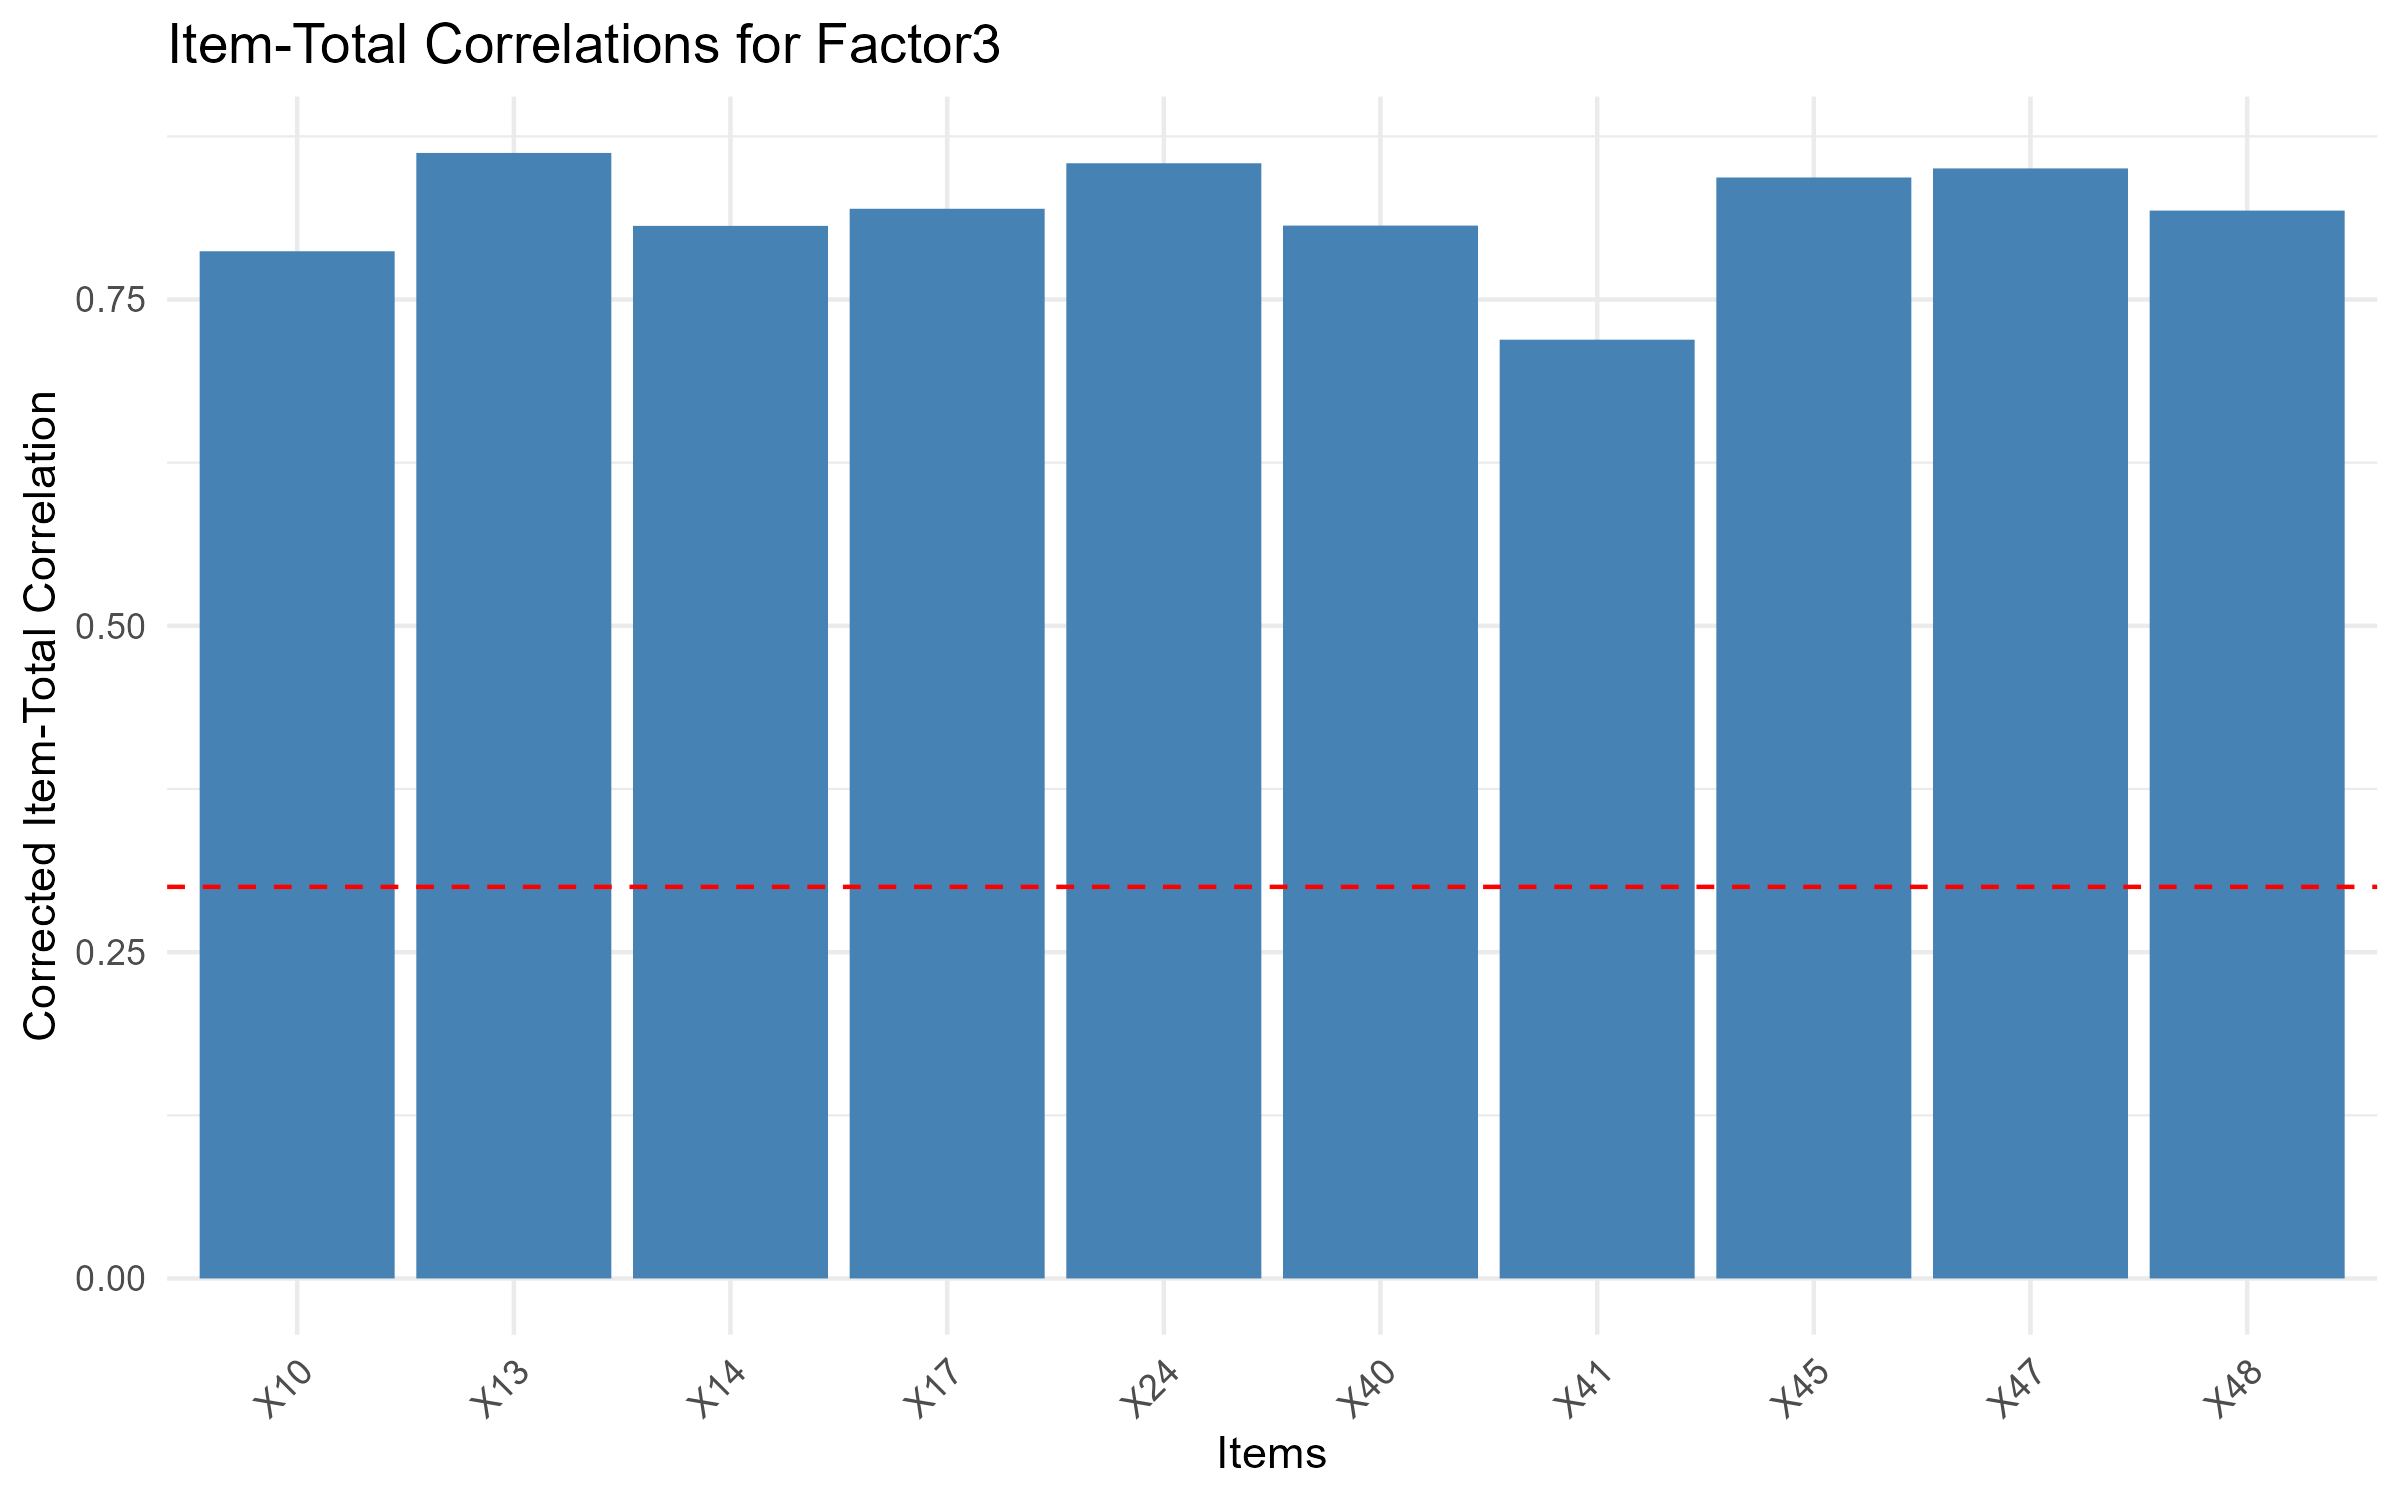
\includegraphics[width=\textwidth]{../../assets/images/reliability_Factor3.png}
        \caption{Độ tin cậy nhân tố 3}
    \end{minipage}
    \hfill
    \begin{minipage}{0.3\textwidth}
        \centering
        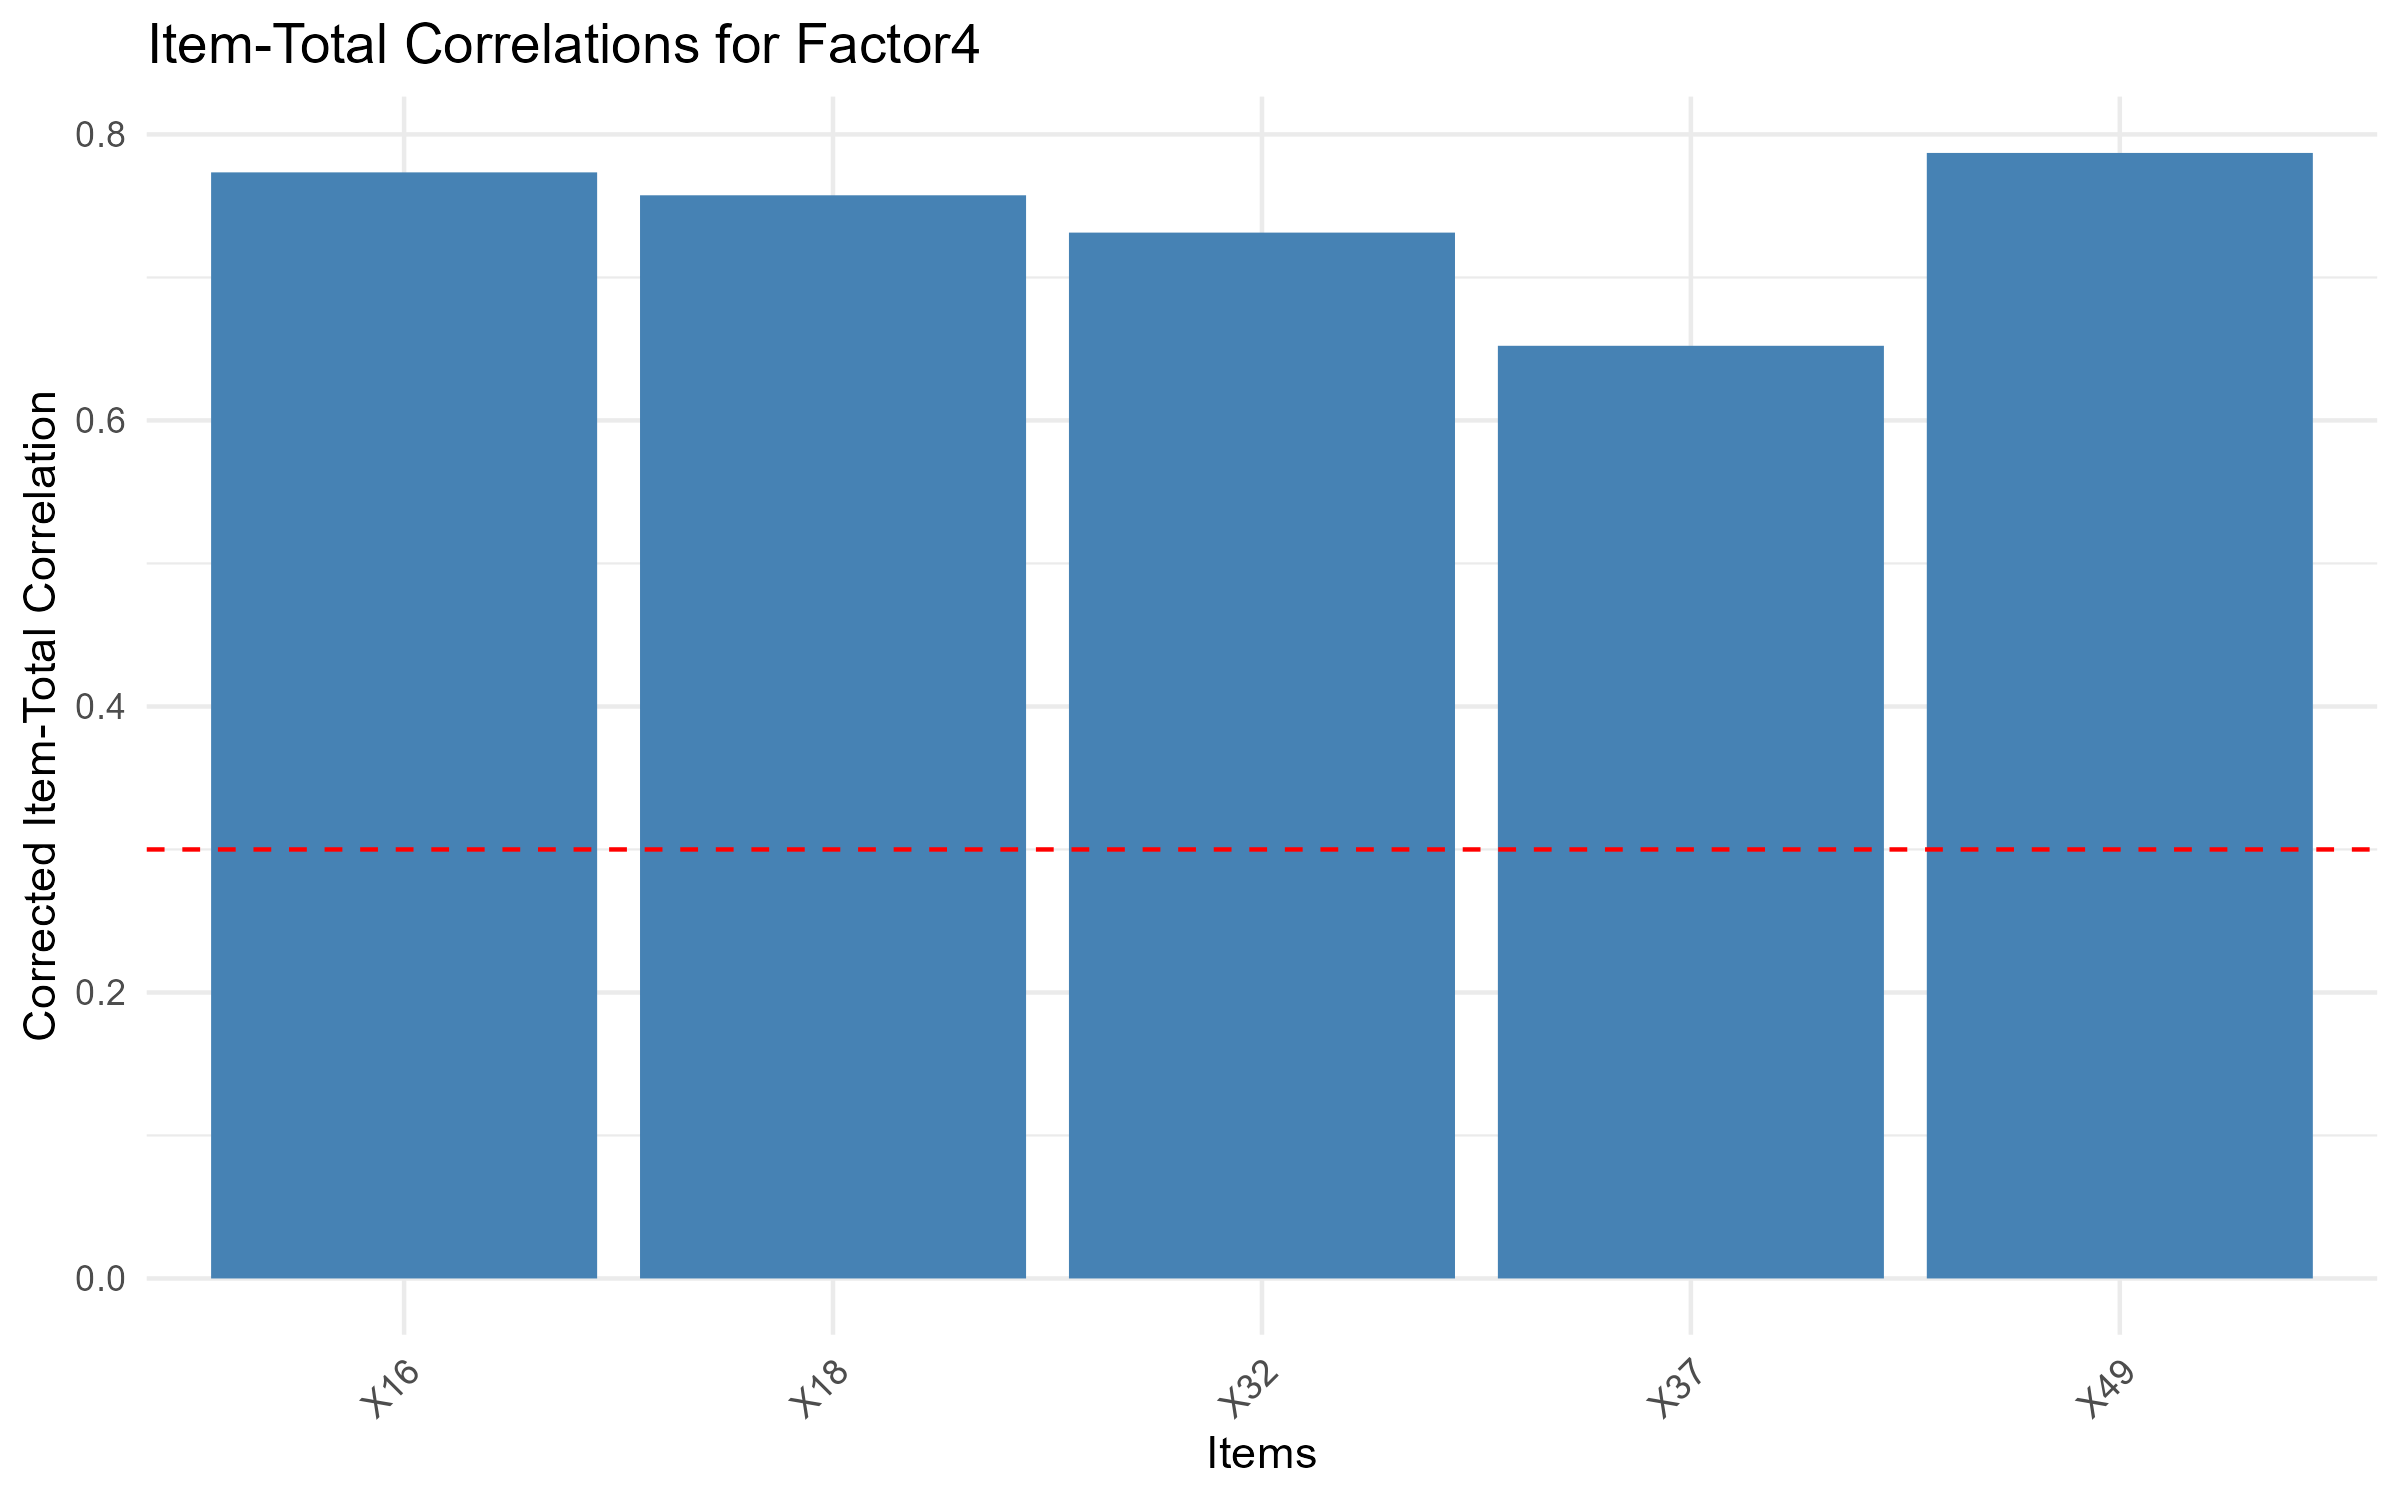
\includegraphics[width=\textwidth]{../../assets/images/reliability_Factor4.png}
        \caption{Độ tin cậy nhân tố 4}
    \end{minipage}
    \hfill
    \begin{minipage}{0.3\textwidth}
        \centering
        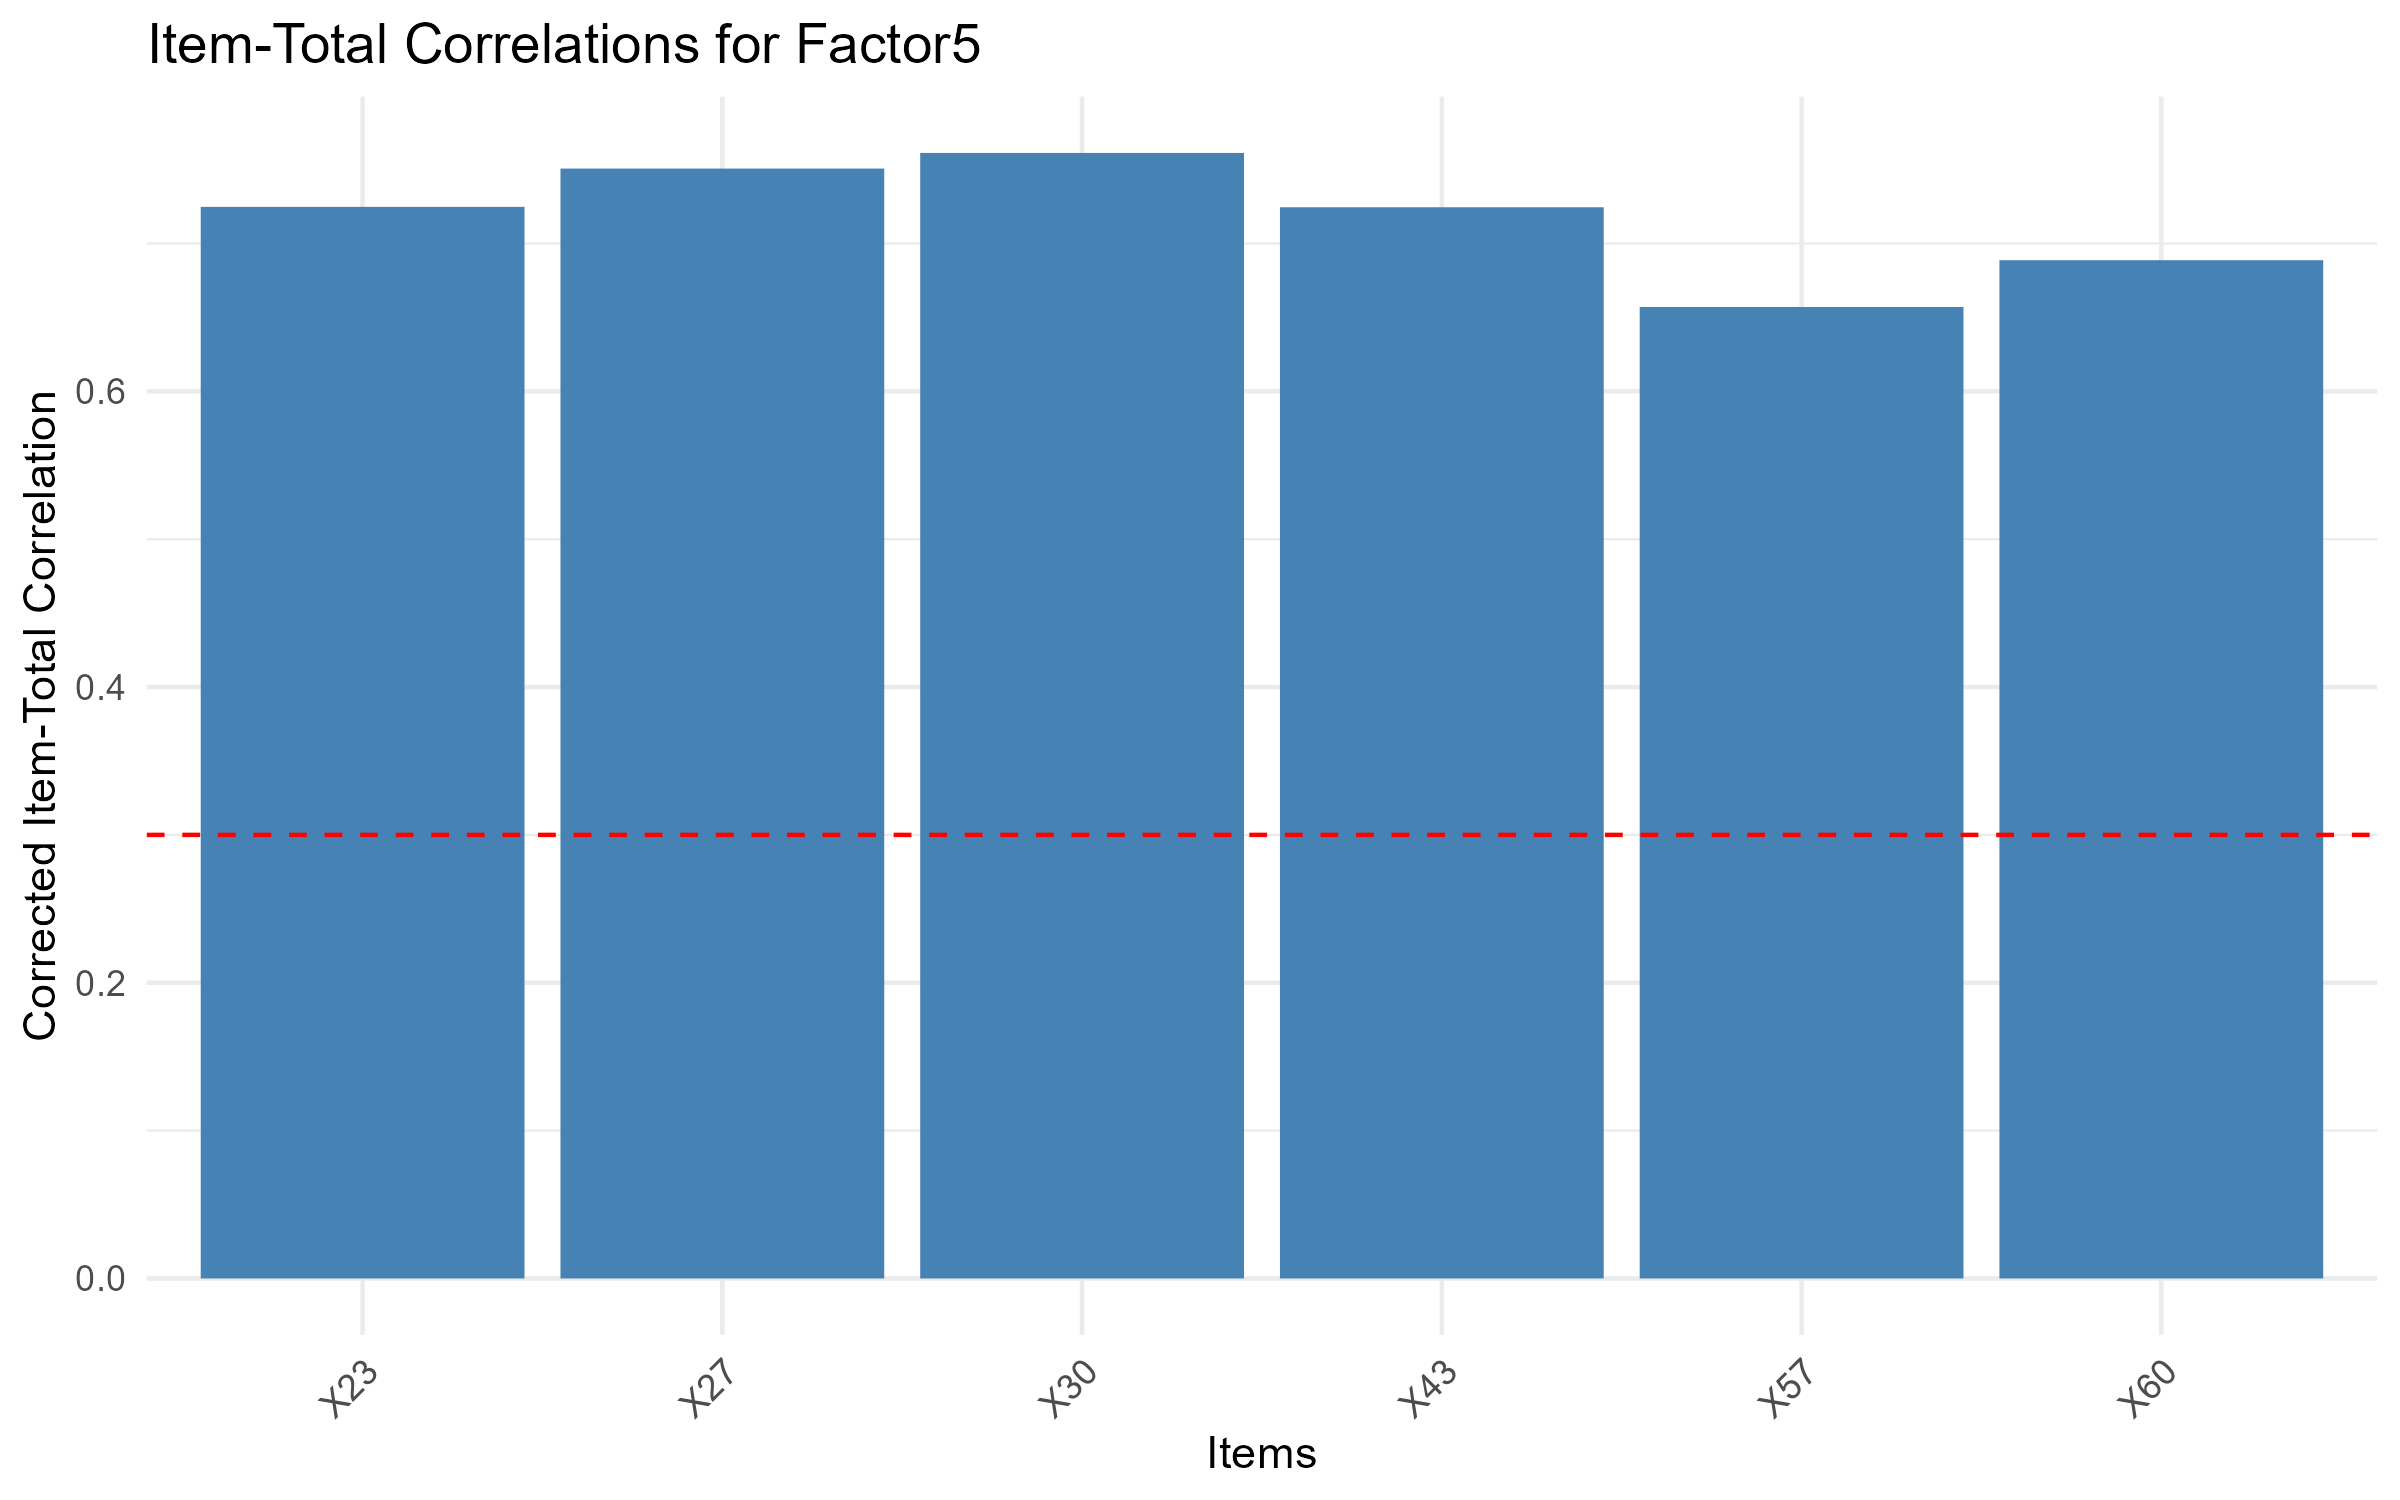
\includegraphics[width=\textwidth]{../../assets/images/reliability_Factor5.png}
        \caption{Độ tin cậy nhân tố 5}
    \end{minipage}
\end{figure}

\section{Phân tích tương quan chính tắc (CCA)}

\subsection{Mô hình CCA}

\begin{matlab}
\begin{lstlisting}
function [A, B, r, U, V] = canonical_correlation_analysis(X, Y)
% CANONICAL_CORRELATION_ANALYSIS
% Thực hiện phân tích tương quan chính tắc giữa hai nhóm biến

% Chuẩn hóa dữ liệu
X = zscore(X);
Y = zscore(Y);

% Tính ma trận tương quan
n = size(X, 1);
Sxx = (X' * X) / (n - 1);
Syy = (Y' * Y) / (n - 1);
Sxy = (X' * Y) / (n - 1);
Syx = Sxy';

% Giải bài toán trị riêng tổng quát
M1 = inv(Sxx) * Sxy * inv(Syy) * Syx;
M2 = inv(Syy) * Syx * inv(Sxx) * Sxy;

[A, D1] = eig(M1);
[B, D2] = eig(M2);

% Sắp xếp theo trị riêng giảm dần
[r, idx] = sort(sqrt(diag(D1)), 'descend');
A = A(:, idx);
B = B(:, idx);

% Tính các biến chính tắc
U = X * A;
V = Y * B;

% Hiển thị kết quả
fprintf('=== PHÂN TÍCH TƯƠNG QUAN CHÍNH TẮC ===\n');
for i = 1:min(3, length(r))
    fprintf('Cặp chính tắc %d: r = %.4f\n', i, r(i));
end

% Kiểm định ý nghĩa thống kê
wilks_lambda = prod(1 - r.^2);
chi2_stat = -(n - 1 - (size(X,2) + size(Y,2) + 1)/2) * log(wilks_lambda);
df = size(X,2) * size(Y,2);
p_value = 1 - chi2cdf(chi2_stat, df);

fprintf('\nKiểm định Wilks Lambda:\n');
fprintf('Lambda = %.4f, Chi2 = %.4f, df = %d, p = %.4f\n', ...
    wilks_lambda, chi2_stat, df, p_value);
end
\end{lstlisting}
\end{matlab}

\begin{figure}[h!]
    \centering
    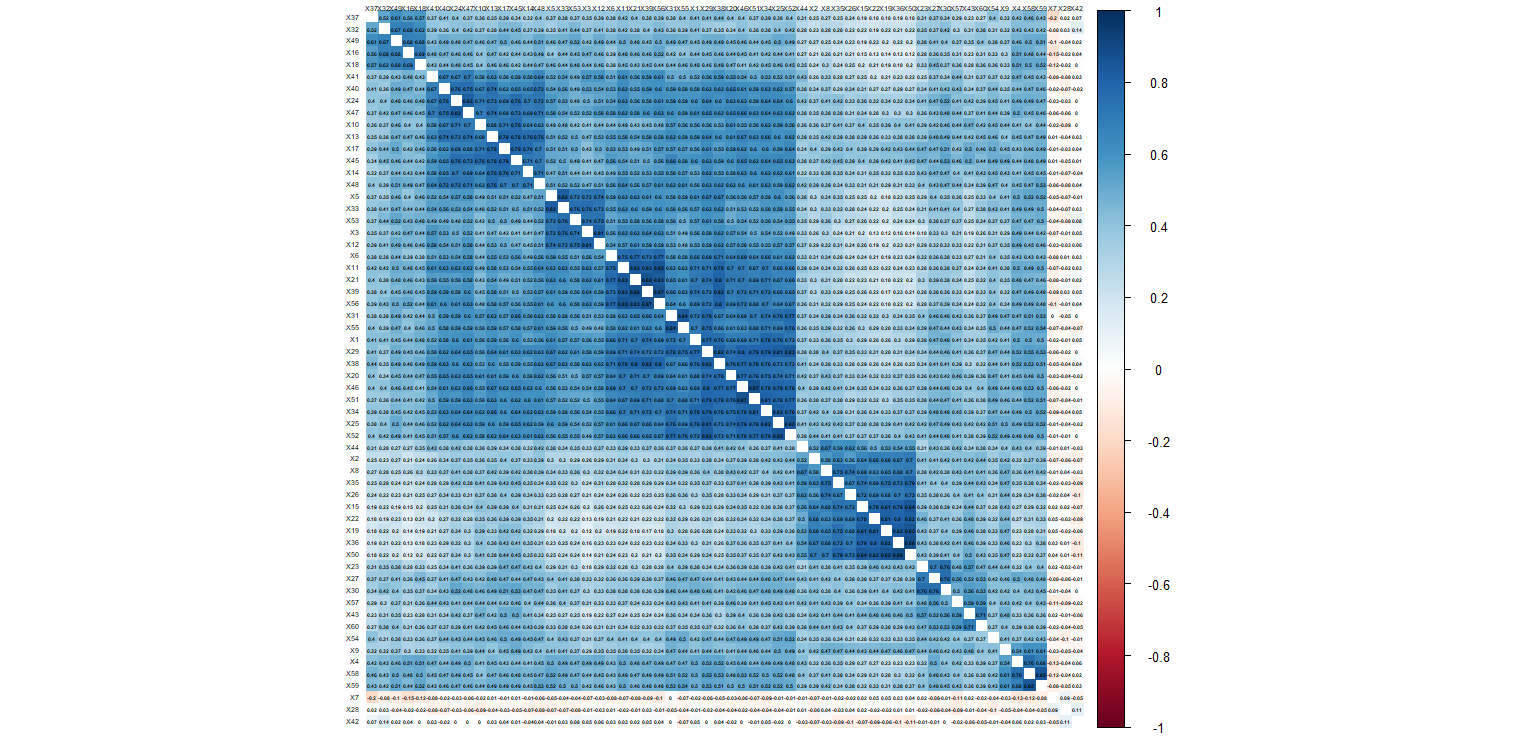
\includegraphics[width=0.8\linewidth]{../../assets/images/correlation_matrix.png}
    \caption{Ma trận tương quan giữa các biến trong phân tích CCA}
\end{figure}

\begin{figure}[h!]
    \centering
    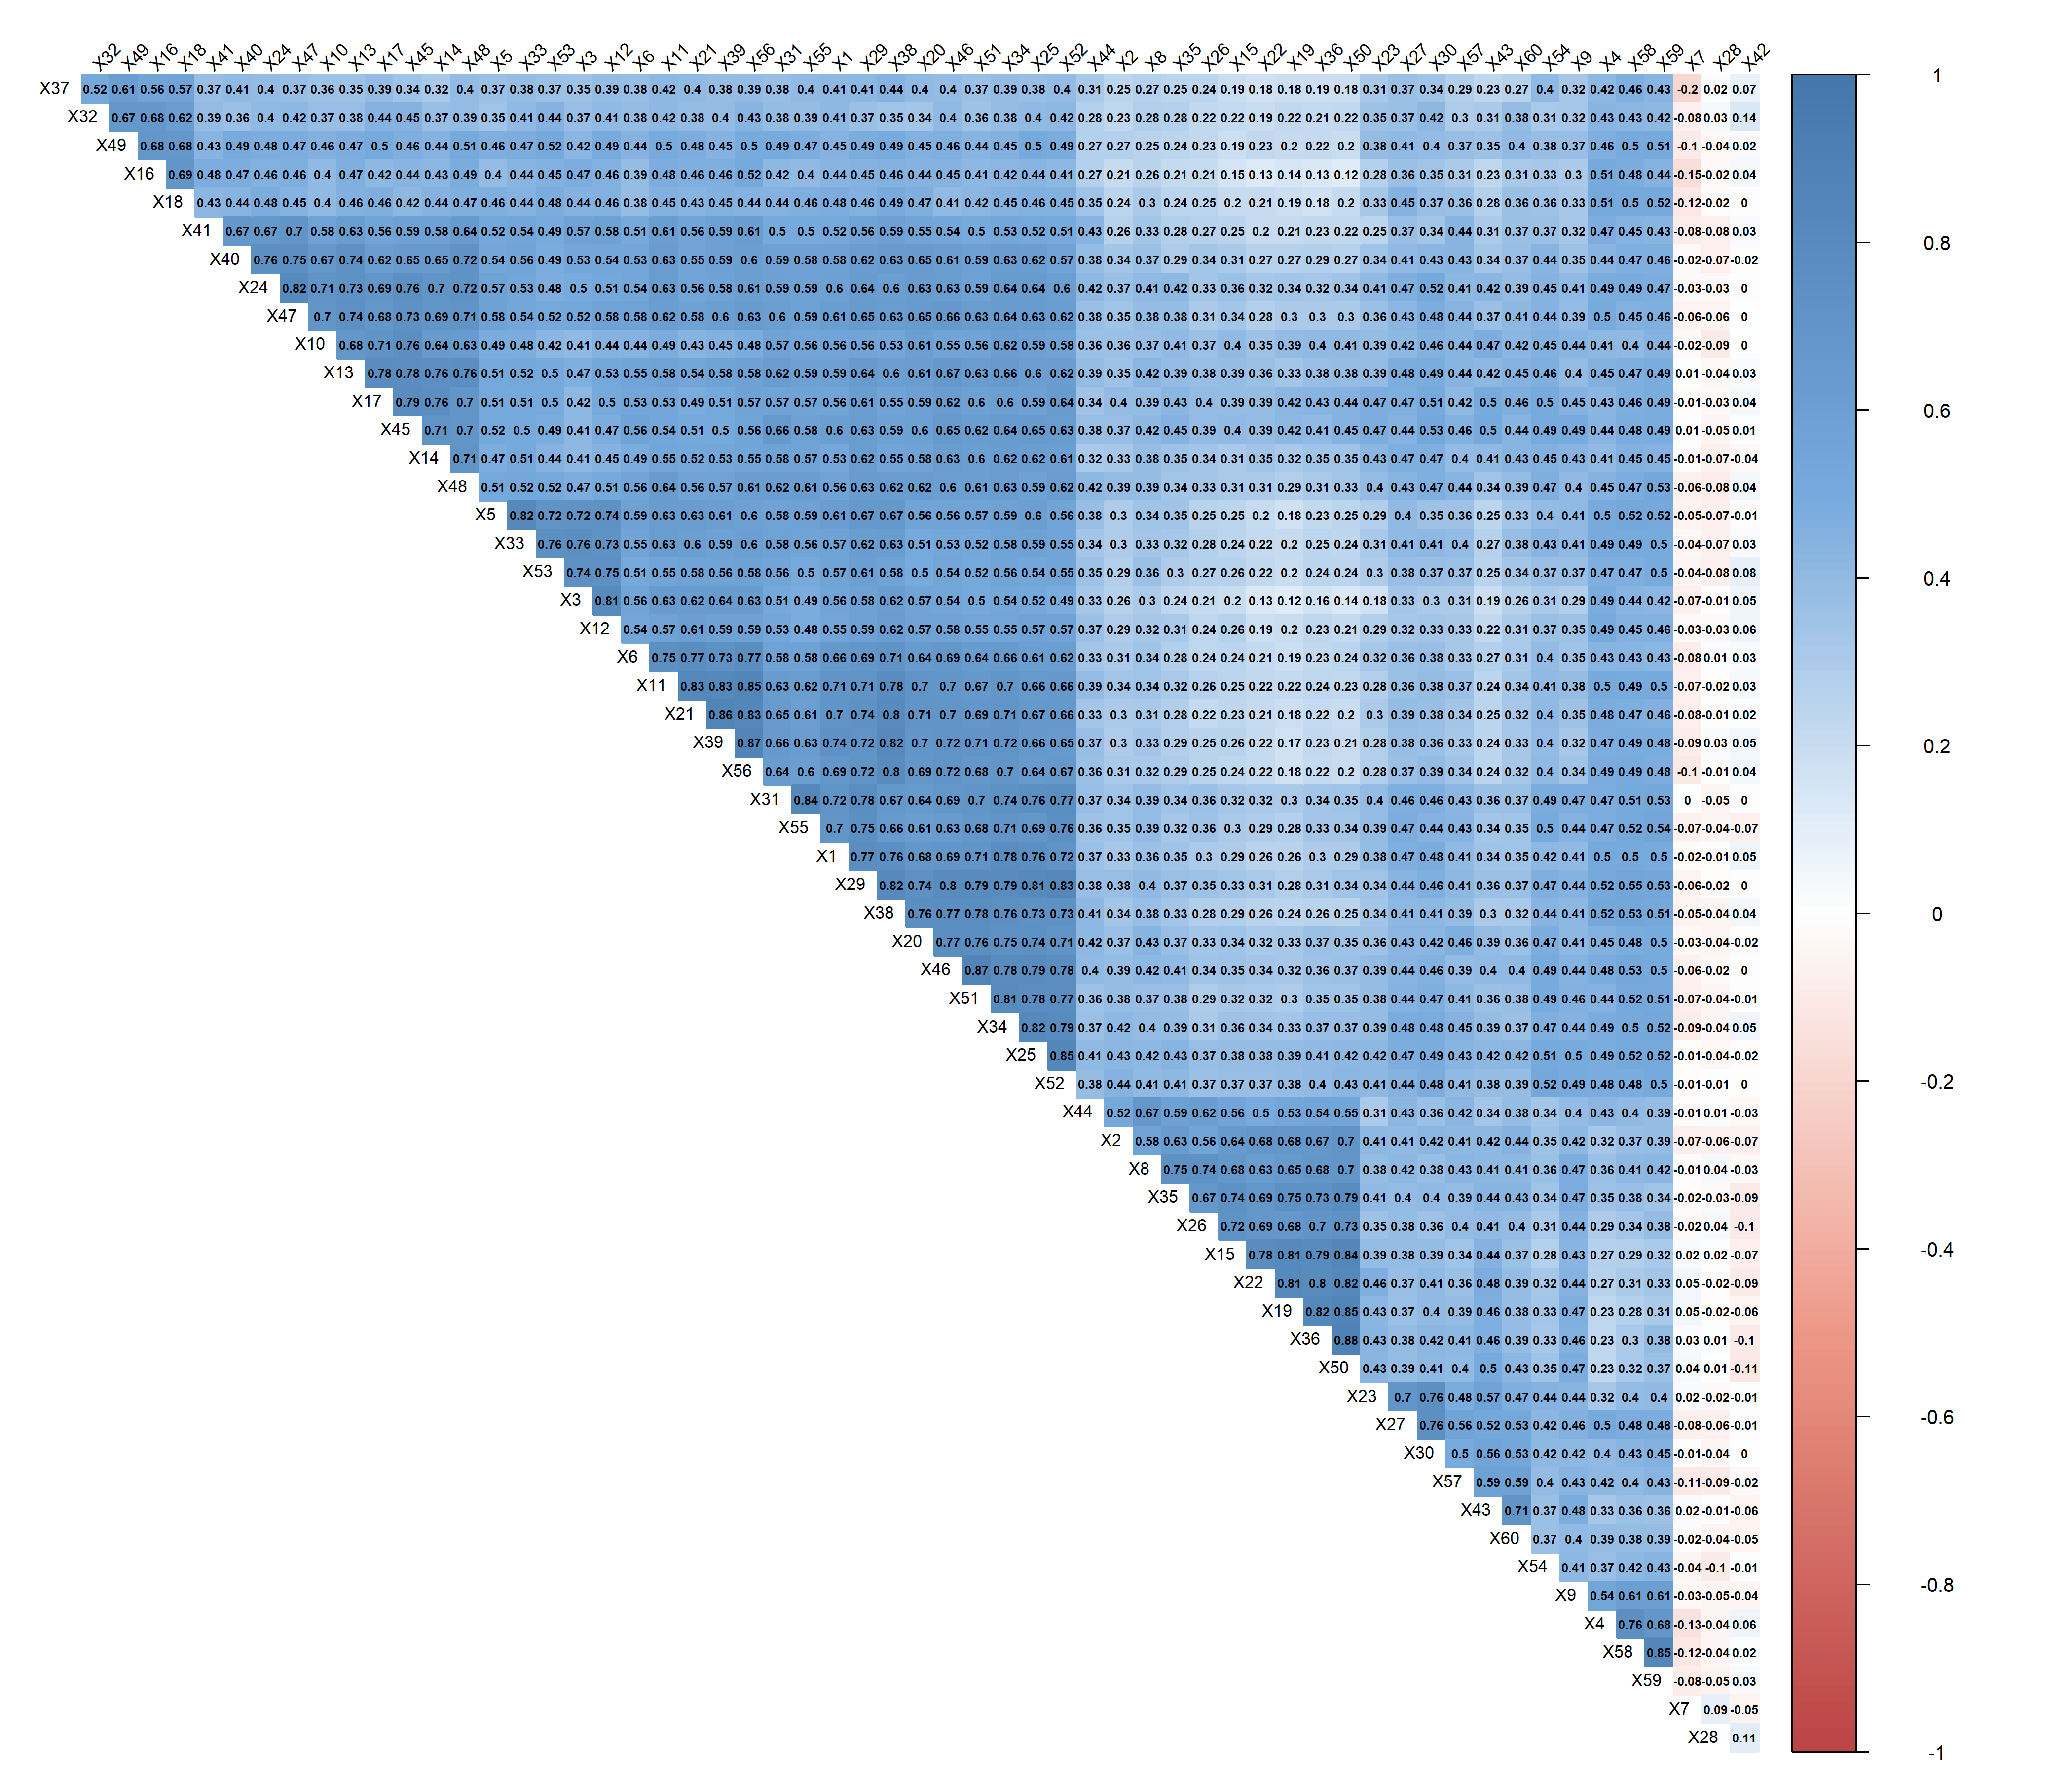
\includegraphics[width=0.8\linewidth]{../../assets/images/correlation_matrix_1.png}
    \caption{Ma trận tương quan chi tiết với các hệ số tương quan}
\end{figure}

\subsection{Kết quả phân tích dữ liệu khác}

\begin{figure}[h!]
    \centering
    \begin{minipage}{0.45\textwidth}
        \centering
        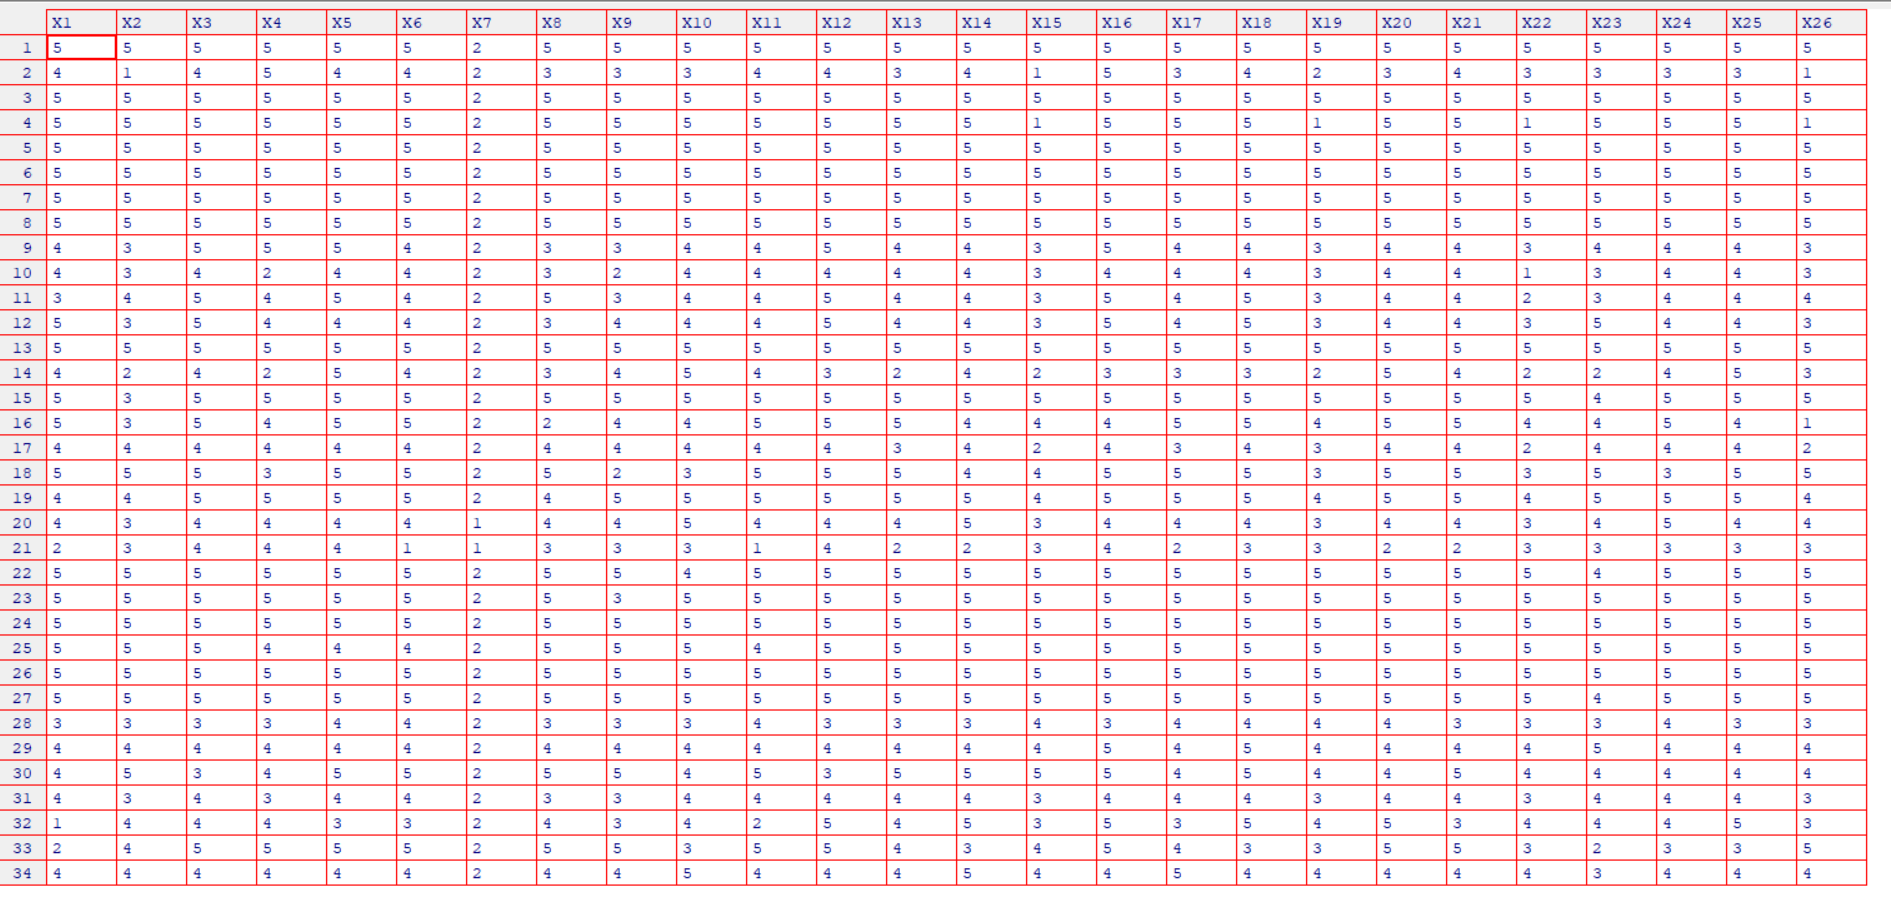
\includegraphics[width=\textwidth]{../../assets/images/data2b.png}
        \caption{Phân tích dữ liệu 2B}
    \end{minipage}
    \hfill
    \begin{minipage}{0.45\textwidth}
        \centering
        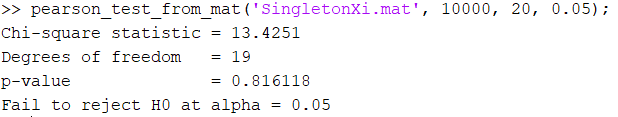
\includegraphics[width=\textwidth]{../../assets/images/chay_singleton.png}
        \caption{Kết quả chạy phân tích Singleton}
    \end{minipage}
\end{figure}

\section{Kết luận chương}

Chương này đã trình bày một cách hệ thống các phương pháp phân tích dữ liệu nhiều chiều quan trọng. Những điểm chính cần ghi nhớ:

\begin{itemize}
    \item \textbf{PCA} phù hợp cho giảm chiều và trực quan hóa dữ liệu
    \item \textbf{Factor Analysis} tập trung vào tìm cấu trúc tiềm ẩn
    \item \textbf{Cluster Analysis} giúp khám phá nhóm tự nhiên trong dữ liệu
    \item \textbf{Discriminant Analysis} hữu ích cho bài toán phân loại có giám sát
    \item Việc kết hợp nhiều phương pháp thường cho hiểu biết sâu sắc hơn về dữ liệu
    \item Cần validation kỹ lưỡng để đảm bảo tính tin cậy của kết quả
\end{itemize}

Các kỹ thuật này tạo thành nền tảng vững chắc cho việc phân tích dữ liệu phức tạp trong thời đại dữ liệu lớn, từ khoa học dữ liệu đến machine learning và các ứng dụng thực tiễn trong nhiều lĩnh vực khác nhau.